\documentclass[pdflatex,sn-mathphys-num]{sn-jnl}
\usepackage{graphicx}%
\usepackage{booktabs}
\usepackage{geometry}
\usepackage{multirow}%
\usepackage{amsmath,amssymb,amsfonts}%
\usepackage{amsthm}%
\usepackage{mathrsfs}%
\usepackage[title]{appendix}%
\usepackage{xcolor}%
\usepackage{textcomp}%
\usepackage{manyfoot}%
\usepackage{algorithmic}
\usepackage[ruled,linesnumbered]
{algorithm2e}
% \usepackage{orcidlink}
\usepackage{listings}
\usepackage{academicons}

\usepackage{hyperref}
\usepackage{tikz}
\usetikzlibrary{backgrounds} %
\usetikzlibrary{arrows.meta,positioning,fit,shapes.multipart,calc}

% Styles (grayscale-friendly)
\tikzset{
  prep/.style={
    rectangle, draw, thick, rounded corners,
    minimum width=4.5cm, minimum height=0.8cm,
    fill=blue!10, font=\footnotesize, align=center
  },
  ai/.style={
    rectangle, draw, thick, rounded corners,
    minimum width=3cm, minimum height=0.7cm,
    fill=green!15, font=\footnotesize, align=center
  },
  dock/.style={
    rectangle, draw, thick, rounded corners,
    minimum width=3.5cm, minimum height=0.9cm,
    fill=orange!15, font=\footnotesize, align=center
  },
  fuse/.style={
    rectangle, draw, thick, rounded corners,
    minimum width=5.5cm, minimum height=1.2cm,
    fill=purple!15, font=\footnotesize, align=center
  },
  eval/.style={
    rectangle, draw, thick, dashed, rounded corners,
    minimum width=3.8cm, minimum height=0.7cm,
    fill=gray!10, font=\footnotesize, align=center
  },
  group/.style={
    rectangle, draw, very thick, rounded corners,
    inner sep=2mm, fill=white, fill opacity=0,
    draw opacity=0.7
  },
  arrow/.style={-{Stealth[scale=0.8]}, thick},
  tap/.style={-{Stealth[scale=0.7]}, thick, dashed}
}
\definecolor{lime}{HTML}{A6CE39}
\DeclareRobustCommand{\orcidicon}{%
    
\begin{tikzpicture}
    \draw[lime, fill=lime] (0,0) 
    circle [radius=0.16] 
    node[white] {{\fontfamily{qag}\selectfont \tiny ID}};
    \draw[white, fill=white] (-0.0625,0.095) 
    circle [radius=0.007];
    \end{tikzpicture}
    \hspace{-2mm}
}

\renewcommand{\orcid}[1]{\href{https://orcid.org/#1}{\textcolor[HTML]{A6CE39}{\orcidicon}}}
\newcommand{\SuppMat}{Supplementary Material}
\newcommand{\SuppFig}[1]{Supplementary Figure~S#1}
\newcommand{\SuppTab}[1]{Supplementary Table~S#1}
\newcommand{\SuppAlg}[1]{Supplementary Algorithm~S#1}
\newcommand{\SuppSec}[1]{Supplementary Section~S#1}

\theoremstyle{thmstyleone}%
\newtheorem{theorem}{Theorem}
\newtheorem{proposition}[theorem]{Proposition}% 

\theoremstyle{thmstyletwo}%
\newtheorem{example}{Example}%
\newtheorem{remark}{Remark}%

\theoremstyle{thmstylethree}%
\newtheorem{definition}{Definition}%

\raggedbottom

\begin{document}

\title[Article Title]{Independent Pseudo-Trajectories as a Null Benchmark for Single-Cell Forecasting}


\author[1]{\fnm{Victor Ikenna} \sur{Kanu}\orcid{0009-0005-5606-8105}}\email{kanuxavier@gmail.com}
\equalcont{These authors contributed equally to this work.}

\author[1]{\fnm{Ihunanya Udodiri} \sur{Ajakwe}\orcid{0009-0004-9922-2320}}\email{ihunanya.ajakwe@gmail.com}
\equalcont{These authors contributed equally to this work.}

\author[1]{\fnm{Josiah Ayoola} \sur{Isong}\orcid{0000-0002-6151-1950}}\email{isongjosiah@gmail.com}
\equalcont{These authors contributed equally to this work.}

\author[2]{\fnm{Simeon Okechukwu} \sur{Ajakwe}\orcid{0000-0002-6973-530X}}\email{simeonajlove@gmail.com}
\equalcont{These authors contributed equally to this work.}

\author*[1]{\fnm{Dong-Seong} \sur{Kim}\orcid{0000-0002-2977-5964}}\email{dskim@kumoh.ac.kr}
\equalcont{These authors contributed equally to this work.}

\affil[1]{\orgdiv{IT Convergence Engineering}, \orgname{Kumoh National Institute of Technology}, \orgaddress{\city{Gumi}, \postcode{39177}, \country{South Korea}}}

\affil[2]{\orgdiv{Smart Computing Department}, \orgname{ Kyungdong University, Global Campus}, \country{South Korea}}


\abstract{\begin{abstract}
\noindent\textbf{Background:} Expressive temporal models such as Transformers, neural ODEs, and physics-informed networks are increasingly used to forecast cell-differentiation states from single-cell RNA-sequencing data. Because these data are cross-sectional snapshots without lineage tracing, forecasts are evaluated on pseudo-trajectories that concatenate independently sampled cells according to a ground-truth stage order. It remains unclear whether these pseudo-trajectories contain learnable temporal structure or if reported model advantages persist under leakage-safe, multi-seed evaluation.
 
\smallskip
\noindent\textbf{Results:} A single leakage-safe protocol was applied to two independent differentiation lineages (dopaminergic and cardiomyocyte) over 20 random seeds, comparing a Transformer against a linear baseline, a complexity-matched random forest, and a mechanistic ODE using paired statistics and an explicit equivalence test. The Transformer was statistically equivalent to both baselines on both lineages; shuffling stage order or removing positional encoding left accuracy unchanged; and fairer ODE calibration monotonically worsened prediction. A previously apparent forecasting advantage arose entirely from train--test leakage and inverted once corrected.
 
\smallskip
\noindent\textbf{Conclusion:} Pseudo-trajectories built from independent cells contain no temporal signal to learn, so added model capacity fits noise rather than dynamics. The leakage-safe, multi-seed, equivalence-tested protocol, with its temporal-order control, generalizes to any single-cell forecasting claim.
\end{abstract}}





\keywords{single-cell RNA-seq, differentiation forecasting, data leakage, equivalence testing, benchmark evaluation}



\maketitle


\section{\textbf{Background}}
\label{sec:intro}

Single-cell RNA sequencing (scRNA-seq) has enabled population-scale characterization of stem-cell differentiation, resolving stage-dependent gene-expression programs across experimental timepoints~\cite{jerber2021population}. A natural ambition is to move from describing these programs to \emph{forecasting} them: given a cell-state representation at early differentiation stages, predict the state at a later stage. Recent work pursues this with increasingly expressive models---neural ordinary differential equations (ODEs) for continuous-time transcriptomic forecasting~\cite{erbe2023transcriptomic}, Transformer architectures for cell-type annotation and large-scale single-cell foundation modelling~\cite{chen2023transformer,cui2024scgpt}, variational-autoencoder--neural-ODE hybrids for lineage-aware trajectory and velocity inference~\cite{farrell2023inferring}, and physics-informed neural stochastic differential equations for learning cellular dynamics under dynamical constraints~\cite{jiang2024physics}. The implicit premise of this progression is that greater model capacity, and in particular the capacity to model temporal dependency, yields better forecasts of differentiation state.

This premise is rarely tested on two fronts that determine whether a reported improvement is real. The first is the structure of the data on which such models are evaluated. Because single-cell measurement is destructive, no cell is observed at more than one timepoint, and a single-cell experiment captures only a static snapshot at one moment, posing a recognised challenge for time-resolved analysis~\cite{la2018rna}. Experimental strategies can partly recover temporal links---metabolic RNA labelling resolves newly transcribed from pre-existing RNA within a cell over hours~\cite{erhard2019scslam,cao2020scifate}, and heritable lineage barcodes connect clonally related cells sampled at different times~\cite{weinreb2020lineage}---but standard cross-sectional differentiation time-courses, including those analysed here, carry neither. For such data, temporal ordering must be imposed computationally, either through pseudotime inference~\cite{saelens2019comparison,haghverdi2016diffusion}, RNA-velocity and dynamical modelling~\cite{la2018rna,bergen2020generalizing}, by optimal-transport couplings that infer probable ancestor--descendant relationships between consecutive time points~\cite{schiebinger2019optimal,lavenant2024toward}, or by assembling \emph{pseudo-trajectories} that concatenate independently sampled cells under a ground-truth stage order. A pseudo-trajectory is not a tracked lineage---its constituent states are statistically independent draws---so it is not obvious that it contains any within-trajectory temporal dependency for a sequence model to exploit. Whether a Transformer's temporal machinery confers any advantage on such data is an empirical question that is seldom posed directly.

The second front is evaluation rigor. Data leakage---the inadvertent sharing of information between training and test partitions---is a pervasive and well-documented failure mode in machine learning applied to biology, producing performance estimates far better than the intended application supports~\cite{whalen2022navigating,bernett2024guiding}. Its reach is not anecdotal: a cross-disciplinary survey attributed irreproducible findings to leakage in at least $294$ papers across $17$ fields, and showed that apparent advantages of complex models over simple baselines frequently fail to reproduce once leakage is removed~\cite{kapoor2023leakage}. In genomics, a common route is preprocessing fitted on the full dataset before splitting---for example normalization, scaling, or feature selection whose parameters are estimated using test samples---so that held-out data silently shape the training inputs~\cite{whalen2022navigating}. Compounding this, model comparisons are often reported from a single random seed, even though both the construction of pseudo-trajectories and the training of neural models are stochastic; a single-seed point estimate cannot separate a genuine effect from sampling variation, motivating community reproducibility efforts that call for repeated runs and reported variance~\cite{pineau2021improving}, and the field's most rigorous benchmarking efforts have instead emphasised many datasets, shared protocols, and reproducible pipelines~\cite{saelens2019comparison}. Establishing that two models perform comparably, moreover, requires an explicit test for equivalence against a pre-specified margin rather than the absence of a significant difference, since a non-significant test is not evidence of equivalence~\cite{lakens2017equivalence}.

Taken together, these two fronts expose a gap: there is no leakage-safe, multi-seed, equivalence-tested benchmark for discrete-stage single-cell differentiation forecasting that also tests, rather than assumes, the presence of the temporal structure that expressive models are designed to capture. Existing evaluations conflate the question ``is this model better?'' with artifacts of how the comparison was constructed. Table~\ref{tab:rigor} summarises the evaluation safeguards relevant to this class of task and the extent to which they are enforced.

This study closes that gap. A single, leakage-safe protocol is applied to two independent differentiation lineages---neural (dopaminergic, iPSC$\rightarrow$dopaminergic neuron)~\cite{jerber2021population} and cardiac (iPSC$\rightarrow$cardiomyocyte)~\cite{elorbany2022single}---reducing scRNA-seq to a compact two-dimensional pluripotency--differentiation state and forecasting the late-stage state from the two earlier stages. Four predictors are evaluated as peers under identical conditions: a linear baseline, a complexity-matched random forest, a Transformer, and a mechanistic ODE calibrated under three regimes of increasing sample-level fidelity. Every comparison is reported over $20$ random seeds that reseed both pseudo-trajectory construction and model training, with paired effect sizes and an explicit equivalence test rather than single-seed point estimates. Dedicated controls---a stage-order shuffle and a positional-encoding ablation---test directly whether the Transformer extracts temporal structure, and a $38$-variant sweep establishes robustness to the state representation.

The findings reframe the apparent value of expressive temporal models in this setting. Under leakage-safe evaluation the Transformer is statistically equivalent to an ten-parameter linear model and to the complexity-matched random forest, on both lineages; destroying stage order leaves its accuracy unchanged; and a fairly calibrated mechanistic model provides no sample-level benefit, degrading monotonically as its calibration is made fairer. A single mechanism accounts for all of these results: pseudo-trajectories built from independently sampled cells contain no temporal dependency to learn, so a memoryless predictor is optimal and additional model capacity fits noise rather than signal. The contribution is therefore less any single negative result than the evaluation protocol that exposes it.

The main contributions are:
\begin{itemize}
    \item A leakage-safe, multi-seed, paired-statistics benchmark for discrete-stage single-cell differentiation forecasting, with an explicit equivalence test, demonstrated on two independent lineages ($40$ seeds total).
    \item A temporal-order control (stage-order shuffle and positional-encoding ablation) that directly tests whether a sequence model exploits temporal structure on pseudo-trajectory data---a diagnostic applicable to any forecasting claim built on cross-sectional snapshots.
    \item A fair three-regime calibration analysis of a mechanistic ODE, quantifying the sample-level value of population-level dynamical priors under increasing calibration fidelity.
    \item A $38$-variant representation-sensitivity analysis establishing that the equivalence is a property of the forecasting task rather than of any particular state construction.
\end{itemize}

\begin{table*}[!htbp]
\centering
\caption{\scriptsize Evaluation rigor of representative prior work on single-cell forecasting and trajectory modelling, relative to the safeguards enforced here. The relevant safeguards are a leakage-safe split (one partition shared across models, preprocessing fit on training data only), multi-seed estimation (repetition across random seeds perturbing data construction and training), an explicit equivalence test (paired effect sizes against a pre-specified margin rather than single-seed point estimates), a temporal-structure control (a direct test, such as order shuffling, of whether temporal dependency is present and used), and cross-lineage replication.}
\label{tab:rigor}
\setlength{\tabcolsep}{6pt}
\renewcommand{\arraystretch}{1.25}
\scalebox{0.75}{
\begin{tabular}{p{2.3cm} p{3.5cm} p{10.2cm}}
\hline \toprule
\textbf{Work} & \textbf{Task focus} & \textbf{Evaluation rigor and gap relative to this study} \\
\midrule
Erbe et al.~\cite{erbe2023transcriptomic} & Continuous-time transcriptomic forecasting (neural ODE) & Forecasts continuous trajectories from paired temporal measurements; single train/test evaluation without multi-seed repetition, equivalence testing, or a temporal-structure control, on one system. \\
\midrule
Chen et al.~\cite{chen2023transformer} & Cell-type annotation (Transformer) & Targets annotation rather than temporal forecasting, so a temporal-structure control is not applicable; reports point performance without multi-seed variance or equivalence testing. \\
\midrule
Cui et al.~\cite{cui2024scgpt} & Single-cell foundation model (Transformer) & Broad multi-dataset pretraining and transfer, but downstream tasks are scored as single-run point estimates without seed-level variance, equivalence testing, or a test of temporal-structure use. \\
\midrule
Farrell et al.~\cite{farrell2023inferring} & Velocity / trajectory inference (VAE + neural ODE) & Infers latent dynamics and lineage-aware trajectories rather than stage-to-stage forecasts under a fixed benchmark split; no leakage-safe shared split, multi-seed estimation, or equivalence testing. \\
\midrule
Jiang and Wan~\cite{jiang2024physics} & Cellular dynamics (physics-informed SDE) & Learns continuous stochastic dynamics under physical constraints; does not quantify mechanistic utility against data-driven baselines under a discrete-stage benchmark, nor report multi-seed or equivalence statistics. \\
\midrule
Saelens et al.~\cite{saelens2019comparison} & Trajectory-inference benchmarking & Establishes leakage-safe, shared-protocol, cross-dataset benchmarking with stability assessment, but targets trajectory/topology recovery rather than forecasting, and does not apply paired equivalence testing or a temporal-structure control. \\
\midrule
\textbf{This study} & \textbf{Discrete-stage differentiation forecasting} & \textbf{Single leakage-safe split shared across all models; 20-seed paired estimation with bootstrap CIs, Wilcoxon tests, and an explicit equivalence margin; a stage-order shuffle and positional-encoding ablation that directly test temporal-structure use; replicated across two lineages.} \\
\hline \toprule
\end{tabular}}
\end{table*}



\begin{figure*}[!htbp]
\centering
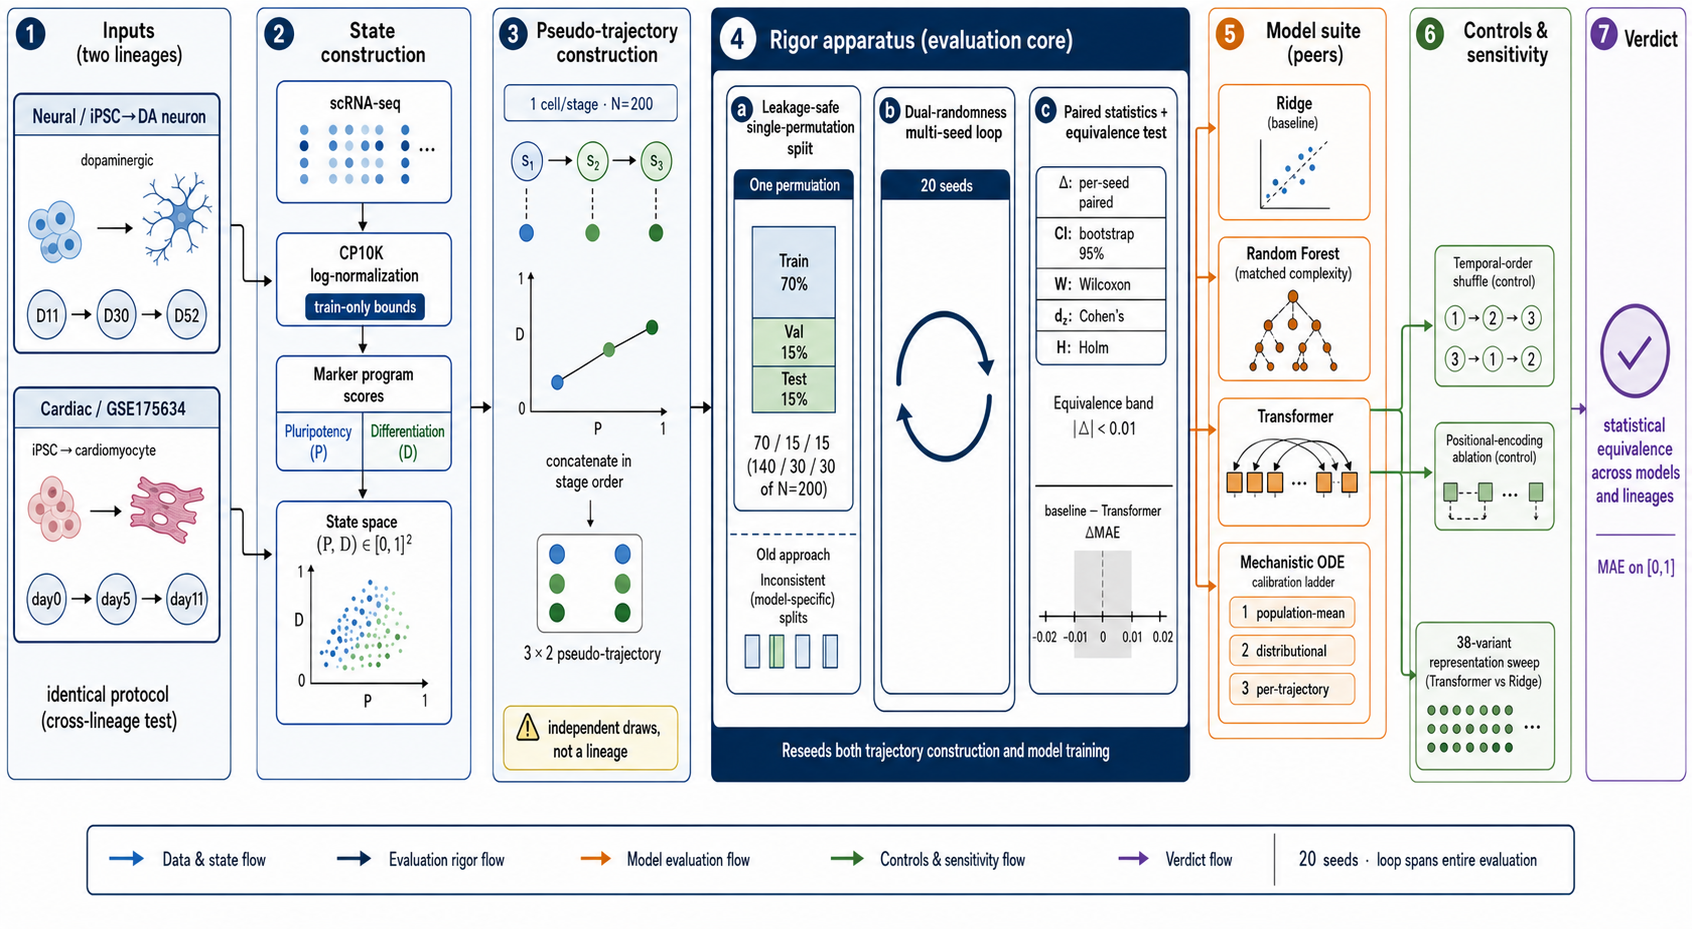
\includegraphics[width=0.99\textwidth]{figures/method_design.png}
\caption{\textbf{Overview of the leakage-safe, multi-seed, equivalence-tested forecasting benchmark.}
An identical protocol is applied to two iPSC differentiation lineages (neural, dopaminergic; cardiac, \texttt{GSE175634}), reducing scRNA-seq to a 2-D pluripotency--differentiation state and assembling stage-ordered pseudo-trajectories ($N=200$ per seed). All models share a leakage-safe $70/15/15$ split, evaluated over $20$ seeds that reseed both trajectory construction and training, and compared by paired $\Delta$MAE with bootstrap CIs, Wilcoxon tests, and an equivalence band $|\Delta|<0.01$. Four predictors (Ridge, complexity-matched random forest, Transformer, mechanistic ODE) are assessed as peers alongside temporal-order and representation controls. Arrow colors denote the data, rigor, model, control, and verdict flows.}
\label{fig:system}
\end{figure*}


\section{\textbf{Methods}}
\label{sec:methods}
The methodology is structured around a single guiding principle: every quantity reported in this study is presented as an estimate with its associated uncertainty, calculated using a protocol that is consistent across all models and eliminates train–test information leakage. This principle determines the organization of the section. Section~\ref{subsec:data_state} details the two differentiation datasets and the reduction of high-dimensional expression data to an interpretable two-dimensional state. Section~\ref{subsec:traj} outlines the pseudo-trajectory construction and explicitly states the underlying assumption, which subsequent controls are designed to test. Section~\ref{subsec:protocol} defines the multi-seed evaluation protocol and the paired statistical methods that replace single-point estimates. Section~\ref{subsec:models} describes the predictors. Sections~\ref{subsec:hybrid} to \ref{subsec:ode_calib} introduce the mechanistic ODE, the hybrid gate that demonstrates its zero marginal utility, and the three calibration regimes that account for this result. Sections~\ref{subsec:controls} to \ref{subsec:sensitivity} present the temporal-structure controls and the representation-sensitivity analysis. Figure~\ref{fig:system} provides an overview of the pipeline.

\subsection{\textbf{Datasets}}
\label{subsec:data_state}

This study deliberately examines two independent differentiation systems rather than one, because a conclusion drawn from a single dataset cannot be distinguished from that dataset's properties. The two systems share a common discrete-stage structure---three ground-truth timepoints, an untreated or control condition, and an identifiable pair of marker programs---but differ in lineage, laboratory of origin, and cell count, which is precisely the variation needed to test whether any finding generalizes. Throughout, each cell is summarized by two scores in $[0,1]$: a pluripotency score $P$ and a lineage-differentiation score $D$, the normalized mean expression of a pluripotency and a differentiation marker panel, respectively (Secs.~\ref{subsec:data_state}--\ref{subsec:state}).

\subsubsection{Neural (dopaminergic) lineage} The neural data are drawn from the population-scale induced-pluripotent-stem-cell (iPSC) to dopaminergic-neuron differentiation resource of~\cite{jerber2021population}, restricted to untreated control samples (treatment $=$ \texttt{NONE}) so that the trajectory reflects unperturbed differentiation. The raw series comprises $205{,}416$ cells across two treatment conditions; after restricting to untreated controls and standard quality control, $161{,}584$ cells are retained across three experimental stages: day~11 (D11, $50{,}661$ cells), day~30 (D30, $50{,}169$ cells), and day~52 (D52, $60{,}754$ cells). These stages span the transition from residual pluripotency through neural progenitor commitment to dopaminergic maturation.

\subsubsection{Cardiac (cardiomyocyte) lineage} As an independent cross-lineage replication, the iPSC$\rightarrow$cardiomyocyte differentiation time-course of~\cite{elorbany2022single} (GEO accession \texttt{GSE175634}) is processed directly from raw counts using the identical pipeline. The deposited series contains $230{,}786$ cells profiled across seven timepoints (days 0, 1, 3, 5, 7, 11, 15) from more than twelve donor lines under a single directed protocol, with no treatment confound; annotation recovers the expected progression from iPSC through mesoderm and progenitor states to cardiomyocyte. The three-stage forecasting task uses day~0, day~5, and day~11 (early iPSC, mid-transition, committed cardiomyocyte; $41{,}330$, $19{,}508$, and $39{,}342$ cells respectively). These stages are chosen deliberately: they span the informative portion of the trajectory while avoiding the post-day-7 plateau, over which the differentiation score is near-constant and would contribute little dynamical signal. This dataset serves specifically to subject every claim made on the neural data to an out-of-distribution test. Before any modeling, the expected developmental biology was confirmed to be recovered under the present state construction: the pluripotency program extinguishes monotonically across the three stages (median $P$: $0.86\!\rightarrow\!0.15\!\rightarrow\!0.00$) and the cardiomyocyte program activates (median $D$: $0.00\!\rightarrow\!0.19\!\rightarrow\!0.22$). This biological sanity check matters because it establishes that a null result on this dataset reflects the structure of the forecasting task rather than a failure to capture differentiation at all.

\subsubsection{Marker programs} Expression is summarized by two curated gene panels per lineage: a pluripotency/progenitor panel $\mathcal{G}_P$ and a lineage-differentiation panel $\mathcal{G}_D$. For the neural data,
\[
\mathcal{G}_P=\{\mathrm{POU5F1,\,NANOG,\,SOX2,\,UTF1,\,TDGF1}\},
\]
\[
\mathcal{G}_D=\{\mathrm{TH,\,DDC,\,SLC6A3,\,DRD2,\,LMX1A,\,FOXA2}\}.
\]
$\mathcal{G}_P$ collects canonical pluripotency transcription factors; $\mathcal{G}_D$ collects dopaminergic-identity and maturation genes spanning dopamine synthesis (\textrm{TH, DDC}), transport (\textrm{SLC6A3}), receptor (\textrm{DRD2}), and floor-plate fate (\textrm{LMX1A, FOXA2}). For the cardiac data the panels are lineage-appropriate analogues, a broadened pluripotency panel and a cardiomyocyte-identity panel:
\[
\mathcal{G}_P^{\mathrm{card}}=\{\mathrm{POU5F1,\,NANOG,\,SOX2,\,LIN28A,\,DPPA4,\,UTF1,\,TDGF1}\},
\]
\begin{align*}
\mathcal{G}_D^{\mathrm{card}}=\{&\mathrm{TNNT2,\,MYH6,\,MYH7,\,ACTC1,\,NPPA,\,MYL7,}\\
&\mathrm{TNNI1,\,TNNI3,\,RYR2,\,NKX2\text{-}5,\,GATA4,\,TBX5,\,MYL2}\}.
\end{align*}
The cardiac differentiation panel spans sarcomeric structure (\textrm{TNNT2, MYH6/7, ACTC1, MYL2/7, TNNI1/3}), calcium handling (\textrm{RYR2}), natriuretic signalling (\textrm{NPPA}), and cardiac transcription factors (\textrm{NKX2-5, GATA4, TBX5}). All base-panel genes were present in their respective datasets with no missing markers. The dopaminergic panel is not transferred onto the cardiac data; doing so would conflate a lineage mismatch with the forecasting question under study. The robustness of all conclusions to the specific choice of genes within each panel is established directly in Sec.~\ref{subsec:sensitivity}.

\subsection{\textbf{State Construction and Leakage-Safe Normalization}}
\label{subsec:state}

For each cell at stage $t$, raw counts are first library-size normalized to $10{,}000$ counts per cell (CP10K) and log-transformed, $\log(1+\mathrm{CP10K})$ (neural data: Scanpy \texttt{normalize\_total}+\texttt{log1p}; cardiac data: the identical transform applied during a single streaming pass over the counts matrix, avoiding loading the full $230{,}786\times 38{,}943$ array). The two state scores are the per-panel means of the log-normalized expression:
\begin{equation}
P^{\mathrm{raw}}_t = \frac{1}{|\mathcal{G}_P|}\sum_{g\in\mathcal{G}_P}\log\!\left(1+\mathrm{expr}_t(g)\right), \quad
D^{\mathrm{raw}}_t = \frac{1}{|\mathcal{G}_D|}\sum_{g\in\mathcal{G}_D}\log\!\left(1+\mathrm{expr}_t(g)\right),
\label{eq:marker_scores}
\end{equation}
with $\mathrm{expr}_t(g)$ the count-depth-normalized expression of gene $g$. Mean-of-log aggregation is chosen for stability and interpretability; Sec.~\ref{subsec:sensitivity} confirms median and $z$-score aggregations give the same conclusions.

Each raw score is min--max scaled to the unit interval using bounds from the training partition only, then clipped:
\begin{equation}
z^{\mathrm{norm}} = \mathrm{clip}\!\left(\frac{z - z_{\min}^{\mathrm{tr}}}{z_{\max}^{\mathrm{tr}} - z_{\min}^{\mathrm{tr}}},\;0,\;1\right), \quad z\in\{P^{\mathrm{raw}},D^{\mathrm{raw}}\}, \quad s_t=[P_t,D_t]\in[0,1]^2,
\label{eq:minmax_clip}
\end{equation}
where $z_{\min}^{\mathrm{tr}},z_{\max}^{\mathrm{tr}}$ are training-cell extrema and $s_t$ is the resulting stage state. Estimating bounds on the full dataset---a common shortcut---would let the held-out range influence preprocessing, a subtle leakage. Clipping mildly compresses values near the lower bound (flattening some medians to zero, or producing a small apparent late-stage uptick); the qualitative trends were verified to persist under unclipped scoring, so clipping affects display range, not dynamics.

\subsection{\textbf{Pseudo-Trajectory Construction and Its Encoded Assumption}}
\label{subsec:traj}

With no lineage tracing across stages---no cell is observed at more than one timepoint---fixed-length sequences are assembled by sampling one cell independently (with replacement) per stage and concatenating their states under ground-truth stage ordering:
\begin{equation}
x^{(i)}=\big[s_{t_0}^{(i)},\,s_{t_1}^{(i)},\,s_{t_2}^{(i)}\big],
\qquad i=1,\dots,N,\;\; N=200,
\label{eq:traj_def}
\end{equation}
giving a $200\times 3\times 2$ tensor per seed.

It is essential to state plainly what this construction does and does not represent, because the interpretation of every downstream result depends on it. Each $x^{(i)}$ is a \emph{population-level pseudo-trajectory}: its three states are independent draws from three marginal stage distributions, stitched together by stage order alone. It is \emph{not} a tracked single-cell lineage. Consequently the only temporal information present in $x^{(i)}$ is the ordering of three otherwise statistically independent samples, and the prediction target $\hat{s}_{t_2}=f(s_{t_0},s_{t_1})$ is a stage-level marker-state distribution rather than the future of any individual cell. This independence has a direct analytical consequence, which defines what any model can achieve on such data.

\begin{proposition}[Independent pairing implies a constant optimal predictor]
\label{prop:null}
Let a test pseudo-trajectory be generated by Eq.~\eqref{eq:traj_def}, so that $s_{t_2}$ is independent of $x=(s_{t_0},s_{t_1})$, and let $f$ be any predictor fitted on training trajectories drawn independently of that test trajectory. Let $m=(m_P,m_D)$ be the component-wise median of the marginal distribution of $s_{t_2}$. Then
\[
\mathbb{E}\big[\mathrm{MAE}_s(f)\big]\;\ge\;\mathbb{E}\big[\mathrm{MAE}_s(m)\big],
\]
with equality only if $f(x)$ is a component-wise median of $s_{t_2}$ for almost every $x$. In particular, $\mathbb{E}[s_{t_2}\mid x]=\mathbb{E}[s_{t_2}]$, and the Bayes-optimal predictor under absolute loss is the constant $m$.
\end{proposition}

\noindent\emph{Proof.} Condition on $x$ and on the training data. The prediction $c=f(x)$ is then fixed, and because $s_{t_2}$ is independent of both, $\mathbb{E}\,|s_{t_2,k}-c_k|$ is minimized, for each component $k\in\{P,D\}$, by any median of the marginal of $s_{t_2,k}$. Averaging over $x$ and the training data gives the inequality. $\square$

Proposition~\ref{prop:null} makes three predictions before any model is trained: (i)~no model can outperform the constant marginal-median predictor in expectation, so models of any capacity can at best tie with one another; (ii)~input transformations that preserve the information about $s_{t_2}$, which is none, such as permuting stage order or removing positional encoding, cannot change attainable accuracy; and (iii)~any input-dependent flexibility, including per-trajectory calibration of a dynamical model, can only add variance. The independently paired benchmark is therefore a \emph{null} setting by construction. The empirical analyses that follow test whether the evaluation protocol correctly recovers this known null, and whether a protocol that lacked these safeguards would instead report a spurious advantage (Sec.~\ref{subsec:res_leakage}). They do not, on their own, establish how models behave when genuine temporal dependence is present.
% TODO(revision): add constant marginal-median baseline to all multi-seed tables/figures,
% and add positive-control experiments (simulated SDE with known coupling; OT-coupled
% pseudo-trajectories) showing the protocol detects an advantage when dependence exists.

Whether a sequence model behaves as Proposition~\ref{prop:null} predicts is checked empirically by the controls in Sec.~\ref{subsec:controls}. This construction is retained precisely because it mirrors what the original study~\cite{kanu2026transformer} and many comparable analyses do, so that the present evaluation speaks to that common practice rather than to an idealized setting.

Algorithm~\ref{alg:traj_norm} formalizes the construction together with the leakage-safe normalization, written as the per-seed procedure actually executed: trajectory sampling, training-only split, training-bounds estimation, and normalization are all driven by a seed that is varied across runs (Sec.~\ref{subsec:protocol}).

\begin{algorithm}[!htbp]
\scriptsize
\caption{\textcolor{black}{Per-Seed Pseudo-Trajectory Construction and Leakage-Safe Normalization}}
\label{alg:traj_norm}
\textbf{Require:} scRNA-seq dataset $\mathcal{X}$ with stage labels $t\in\{t_0,t_1,t_2\}$, untreated/control filter $\phi(\cdot)$, marker panels $\mathcal{G}_P,\mathcal{G}_D$, trajectory count $N=200$, split sizes $(N_{\mathrm{tr}},N_{\mathrm{val}},N_{\mathrm{te}})=(140,30,30)$, seed $s$ \\
\textbf{Output:} Trajectories $\mathcal{T}=\{x^{(i)}\}_{i=1}^{N}$, split indices $(\mathcal{I}_{\mathrm{tr}},\mathcal{I}_{\mathrm{val}},\mathcal{I}_{\mathrm{te}})$, training bounds $\mathcal{B}$ \\
\BlankLine
\textbf{SetSeed}$(s)$ \tcp*{seed governs sampling \emph{and} split}
\tcp{Filter to untreated/control and partition by ground-truth stage}
$\mathcal{X}_0 \leftarrow \{x\in\mathcal{X}\;:\;\phi(x)=1\}$ \;
$\mathcal{X}_{t}\leftarrow \{x\in\mathcal{X}_0: \mathrm{stage}(x)=t\}$ \textbf{ for } $t\in\{t_0,t_1,t_2\}$ \;
\BlankLine
\tcp{Sample independent cells per stage and form ordered pseudo-trajectories}
\For{$i\leftarrow 1$ \KwTo $N$}{
    \For{$t \in \{t_0,t_1,t_2\}$}{
        $c_t \sim \mathcal{U}(\mathcal{X}_t)$ \tcp*{independent draw}
        $P^{\mathrm{raw}}_t\leftarrow \frac{1}{|\mathcal{G}_P|}\sum_{g\in\mathcal{G}_P}\log(1+\mathrm{expr}_{c_t}(g))$ \;
        $D^{\mathrm{raw}}_t\leftarrow \frac{1}{|\mathcal{G}_D|}\sum_{g\in\mathcal{G}_D}\log(1+\mathrm{expr}_{c_t}(g))$ \;
    }
    $x_{\mathrm{raw}}^{(i)}\leftarrow \big[(P^{\mathrm{raw}}_{t_0},D^{\mathrm{raw}}_{t_0}),(P^{\mathrm{raw}}_{t_1},D^{\mathrm{raw}}_{t_1}),(P^{\mathrm{raw}}_{t_2},D^{\mathrm{raw}}_{t_2})\big]$ \;
    $\mathcal{T}_{\mathrm{raw}}\leftarrow \mathcal{T}_{\mathrm{raw}}\cup\{x_{\mathrm{raw}}^{(i)}\}$ \;
}
\BlankLine
\tcp{Trajectory-level split, shared identically across all models}
$(\mathcal{I}_{\mathrm{tr}},\mathcal{I}_{\mathrm{val}},\mathcal{I}_{\mathrm{te}})\leftarrow \textbf{SplitIndices}(N,N_{\mathrm{tr}},N_{\mathrm{val}},N_{\mathrm{te}})$ \;
\BlankLine
\tcp{Min--max bounds from TRAINING trajectories only (prevents leakage)}
$\mathcal{S}_{\mathrm{tr}}\leftarrow \{(P^{\mathrm{raw}},D^{\mathrm{raw}})\in x_{\mathrm{raw}}^{(i)}: i\in \mathcal{I}_{\mathrm{tr}}\}$ \;
$P_{\min/\max}^{\mathrm{tr}}\leftarrow \min/\max \mathcal{S}_{\mathrm{tr}}(P^{\mathrm{raw}})$;\quad
$D_{\min/\max}^{\mathrm{tr}}\leftarrow \min/\max \mathcal{S}_{\mathrm{tr}}(D^{\mathrm{raw}})$ \;
$\mathcal{B}\leftarrow \{P_{\min}^{\mathrm{tr}},P_{\max}^{\mathrm{tr}},D_{\min}^{\mathrm{tr}},D_{\max}^{\mathrm{tr}}\}$ \;
\BlankLine
\tcp{Normalize all trajectories with training bounds and clip to $[0,1]$}
\For{$i\leftarrow 1$ \KwTo $N$}{
    \ForEach{$(P^{\mathrm{raw}},D^{\mathrm{raw}})\in x_{\mathrm{raw}}^{(i)}$}{
        $P\leftarrow \mathrm{clip}\!\big(\tfrac{P^{\mathrm{raw}}-P_{\min}^{\mathrm{tr}}}{P_{\max}^{\mathrm{tr}}-P_{\min}^{\mathrm{tr}}},0,1\big)$;\quad
        $D\leftarrow \mathrm{clip}\!\big(\tfrac{D^{\mathrm{raw}}-D_{\min}^{\mathrm{tr}}}{D_{\max}^{\mathrm{tr}}-D_{\min}^{\mathrm{tr}}},0,1\big)$ \;
        Replace $(P^{\mathrm{raw}},D^{\mathrm{raw}})$ with $(P,D)$ in $x^{(i)}$ \;
    }
    $\mathcal{T}\leftarrow \mathcal{T}\cup\{x^{(i)}\}$ \;
}
\BlankLine
\Return $(\mathcal{T},\mathcal{I}_{\mathrm{tr}},\mathcal{I}_{\mathrm{val}},\mathcal{I}_{\mathrm{te}},\mathcal{B})$
\end{algorithm}

\subsection{\textbf{Multi-Seed Evaluation Protocol and Statistics}}
\label{subsec:protocol}

\subsubsection{Forecasting task and metric} The task maps the two earliest stage states to the latest, $\hat{s}_{t_2}=f(s_{t_0},s_{t_1})$, scored by mean absolute error averaged over the two state components:
\begin{equation}
\mathrm{MAE}=\frac{1}{n}\sum_{i=1}^{n}\big|y^{(i)}-\hat{y}^{(i)}\big|, \qquad
\mathrm{MAE}_{s}=\tfrac{1}{2}\big(\mathrm{MAE}_{P}+\mathrm{MAE}_{D}\big).
\label{eq:mae}
\end{equation}
A secondary diagnostic of temporal robustness trains on the early transition and tests on the late one ($x_{t_0:t_1}\!\rightarrow\!s_{t_1}$ vs.\ $x_{t_1:t_2}\!\rightarrow\!s_{t_2}$) under identical preprocessing.

\paragraph{Why a single seed is insufficient:} The pseudo-trajectory construction and model training are both stochastic, and a single fixed seed yields one realization from the joint distribution over both. Reporting that one realization as a point estimate gives no indication of its variability and, as the Results show, can be dominated by it. MAE is therefore treated as a random variable whose distribution is estimated directly.

\subsubsection{Seeds perturb both randomness sources.} The protocol runs $S=20$ seeds. Each seed perturbs \emph{both} (i) pseudo-trajectory construction---which cells are sampled and how they are paired and split, via Algorithm~\ref{alg:traj_norm}---and (ii) model training: weight initialization, dropout masks, and minibatch ordering for the Transformer, and bootstrap resampling for the Random Forest. For each seed a single canonical $140/30/30$ split is drawn and shared identically by every model, so that for any pair of models the difference in MAE on a given seed is a genuine paired observation on the same data.

\subsubsection{A single consistent split, by permutation} Within each seed, the $N=200$ trajectory indices are permuted with the seed's random number generator and partitioned $70/15/15$ ($140$ train, $30$ validation, $30$ test). The permutation is applied once and the resulting index sets are used identically by every model, so that the partitions are mutually disjoint and no trajectory appears in more than one of them. This single-permutation protocol eliminates, by construction, the train–test overlap that arises when a permuted training set is paired with a contiguously sliced test set, the effect of which is quantified in Sec.~\ref{subsec:res_leakage}.

\subsubsection{Paired statistics and effect sizes} Each model is summarized by its across-seed mean, standard deviation, and $95\%$ confidence interval of MAE. Each baseline is compared to the Transformer via the per-seed paired difference $\Delta^{(s)} = \mathrm{MAE}^{(s)}_{\text{baseline}} - \mathrm{MAE}^{(s)}_{\text{Transformer}}$, summarized by three quantities: a percentile paired-bootstrap $95\%$ CI on $\overline{\Delta}$ ($10^4$ resamples), a Wilcoxon signed-rank test (no normality assumption, appropriate at $S=20$), and the standardized effect size $d_z=\overline{\Delta}/\mathrm{sd}(\Delta)$. With multiple baselines, $p$-values are Holm--Bonferroni corrected. Effect size and CI placement are weighted over nominal significance. Following the two-one-sided-tests logic~\cite{lakens2017equivalence}, two models are declared \emph{equivalent} only when the entire $95\%$ CI on $\overline{\Delta}$ lies within the pre-specified margin $|\Delta|<\delta$, with $\delta=0.01$ MAE units (roughly half the seed-to-seed standard deviation of MAE). A CI that merely contains zero, or a non-significant Wilcoxon test, is \emph{not} taken as evidence of equivalence: it indicates only that no difference was detected. This distinction is what permits a defensible negative claim rather than a mere failure to reject.

\subsection{\textbf{Predictive Models}}
\label{subsec:models}

\subsubsection{Classical baselines} Two predictors operate on the flattened two-stage context $x=[P_{t_0},D_{t_0},P_{t_1},D_{t_1}]\in\mathbb{R}^4$ to predict $\hat{s}_{t_2}\in\mathbb{R}^2$. \emph{Ridge regression} ($\alpha=1.0$) is a linear map $\hat{s}_{t_2}=Wx+b$ with $\ell_2$ regularization and ten free parameters ($W\in\mathbb{R}^{2\times4}$, $b\in\mathbb{R}^2$); it is the baseline-of-record because it is the simplest model that can express a smooth dependence of the late state on the early states. \emph{Random Forest} operates on the same representation, included to test whether nonlinear capacity \emph{without} sequence structure improves prediction. In the multi-seed experiments it is complexity-matched by tuning per seed with 3-fold cross-validation on the training partition only (300 trees; maximum depth $\in\{2,3,5,\text{unbounded}\}$; minimum samples per leaf $\in\{1,5,10\}$; MAE scoring). The single-seed leakage analysis (Sec.~\ref{subsec:res_leakage}) reproduces the original fixed configuration (100 trees, maximum depth 10, minimum samples per split 5).

\subsubsection{Transformer} The encoder treats $[s_{t_0},s_{t_1}]$ as a length-two token sequence (each token a 2D state), projecting tokens to $d_{\mathrm{model}}$ dimensions with a fixed sinusoidal positional encoding and emitting the prediction from an MLP head applied to the encoder output at the final position:
\begin{equation}
h_t = W_e s_t + b_e + \mathrm{PE}(t), \qquad
\hat{s}_{t_2} = \mathrm{MLP}\big(\mathrm{Enc}([h_{t_0},h_{t_1}])_{t_1}\big),
\label{eq:transformer}
\end{equation}
with $W_e\in\mathbb{R}^{d_{\mathrm{model}}\times 2}$, $\mathrm{Enc}(\cdot)$ the stacked self-attention encoder, and $\mathrm{MLP}$ a two-layer GELU network. Configuration: input projection $\mathbb{R}^2\!\rightarrow\!d_{\mathrm{model}}{=}128$, 4 encoder layers, 8 attention heads, feedforward dimension 512, GELU, dropout 0.1, MLP head ($128\!\rightarrow\!256\!\rightarrow\!2$, GELU, dropout 0.1) read from the final position ($\approx$827K parameters); Adam ($10^{-3}$, weight decay $10^{-5}$), MSE loss, batch 32, gradient-norm clip 1.0, \texttt{ReduceLROnPlateau} (factor 0.5, patience 10), up to 100 epochs with best-validation selection. The positional encoding and the self-attention over the two stages are the only routes by which temporal order enters; Sec.~\ref{subsec:controls} tests exactly these.

\subsubsection{Mechanistic ODE} A continuous-time, two-state model describes the differentiation programs in calendar time:
\begin{align}
\frac{dP}{dt} &= k_{ps}(1-P) - k_{pd}P - rPD,
\label{eq:ode_p}\\
\frac{dD}{dt} &= k_b + k_{ds}PD + rPD - k_{dd}D,
\label{eq:ode_d}
\end{align}
where $k_{ps}$ maintains $P$, $k_{pd}$ decays it, $k_b$ basally induces $D$, $k_{ds}$ couples $D$-synthesis to $P$, $k_{dd}$ decays $D$, and $r$ sets commitment coupling via $PD$. To stay parameter-frugal and identifiable from three timepoints, $k_{ps}{=}1.0$ and $k_{dd}{=}0.3$ are fixed and four parameters $[k_{pd},k_{ds},r,k_b]$ are free, bounded to $[0,2]^3\times[0,1]$. Integration uses \texttt{solve\_ivp} (RK45, \texttt{rtol}~$10^{-4}$, \texttt{atol}~$10^{-6}$) over the inter-stage calendar intervals---$t=[0,19,41]$ d (neural) and $t=[0,5,11]$ d (cardiac)---with outputs clipped to $[0,1]$ for comparability.

\subsection{\textbf{Hybrid Gated Fusion: Testing Marginal Mechanistic Value}}
\label{subsec:hybrid}

Before asking whether the ODE can be calibrated to compete, a prior question is whether any mechanistic correction is selected at all given the best data-driven prediction. A gated fusion combines the frozen Transformer ($\hat{y}_{\mathrm{ML}}$) and frozen calibrated ODE ($\hat{y}_{\mathrm{phys}}$) through a learnable state-dependent gate $\lambda(x)$, trained with $\ell_1$ sparsity while both predictors stay frozen:
\begin{equation}
\hat{y}_{\mathrm{hyb}} = \hat{y}_{\mathrm{ML}} + \lambda(x)\big(\hat{y}_{\mathrm{phys}} - \hat{y}_{\mathrm{ML}}\big), \qquad
\mathcal{L}_{\lambda} = \frac{1}{n}\sum_{i}\big\|y^{(i)}-\hat{y}^{(i)}_{\mathrm{hyb}}\big\|_2^2 + \frac{\alpha}{n}\sum_{i}\big|\lambda(x^{(i)})\big|,
\label{eq:hybrid}
\end{equation}
where $\lambda(x)=\sigma(g(x))\in[0,1]$ is an MLP ($2\!\rightarrow\!16\!\rightarrow\!8\!\rightarrow\!1$, ReLU/sigmoid) on $x=[P,D]$ and $\alpha=0.01$. The limits are interpretable: $\lambda\!\approx\!0$ recovers the Transformer, $\lambda\!\approx\!1$ the ODE, so the learned gate reads as the data's preference. A gate collapsing toward zero means the data assign negligible weight to the mechanistic prediction. Because that outcome invites the objection of unfair calibration, the next subsection removes it.

\subsection{\textbf{Fair ODE Calibration Under Three Regimes}}
\label{subsec:ode_calib}

The four free parameters are fit by differential evolution under three regimes of increasing sample-level fairness, separating whether the ODE \emph{can} fit the data from whether fitting it more faithfully \emph{helps}:
\begin{enumerate}
    \item \textbf{Population-mean.} Fit once so that integrating from the training-mean $t_0$ state reproduces the training-mean states at $t_1,t_2$, minimizing $\mathcal{L}_{\mathrm{cal}}(\theta)=\sum_{t\in\{t_1,t_2\}}\lVert\tilde{s}_t(\theta)-\bar{s}_t\rVert_2^2$. A population-trend baseline only.
    \item \textbf{Distributional.} Fit so a simulated ensemble (propagating a 40-point subsample of the training $t_0$ distribution) matches both the \emph{mean and standard deviation} at $t_1,t_2$, reducing the population--sample mismatch.
    \item \textbf{Per-trajectory.} Fit per test trajectory (initialized at the population fit) to reproduce its own $t_0\!\rightarrow\!t_1$ step, then integrated onward to $t_2$---the most generous sample-level use.
\end{enumerate}
Each calibrated ODE is evaluated on the identical held-out trajectories. The design licenses a conclusion about mechanistic priors in general: if fairer sample-level calibration does not improve held-out prediction, the limitation is the prior, not the fit.

\subsection{\textbf{Temporal-Structure Controls}}
\label{subsec:controls}

Because the pseudo-trajectories pair independently sampled cells (Sec.~\ref{subsec:traj}), the question of whether the Transformer uses temporal structure cannot be settled by its architecture; it must be measured. Two controls are applied on both datasets across all 20 seeds, each compared to the ordered model with the paired statistics of Sec.~\ref{subsec:protocol}:
\begin{itemize}
    \item \textbf{Stage-order shuffle.} Only the two \emph{input} stages are affected; the target $s_{t_2}$ is never moved. For each trajectory, a random permutation of its two input tokens $[s_{t_0},s_{t_1}]$ is drawn once (seeded per run) and applied before training and evaluation, so that each trajectory's inputs are independently either kept in order or swapped (each with probability $1/2$). The same rule is applied to the training, validation, and test partitions. Stage values are preserved; only their consistent ordering is destroyed, so the model can no longer rely on a given position holding the earlier stage. If the model is genuinely exploiting temporal ordering, destroying that ordering should degrade performance; if MAE is statistically unchanged, the ordering carried no usable signal.
    \item \textbf{Positional-encoding ablation.} The sinusoidal $\mathrm{PE}(t)$ term is removed, disabling the explicit temporal index while leaving model capacity intact. An unchanged MAE indicates that positional information contributes nothing.
\end{itemize}
Together these isolate the two channels through which temporal order can affect the prediction. They constitute the decisive test of whether ``forecasting'' is a meaningful description of the task on pseudo-trajectory data, and their results are reported as equivalence statements (CI on the paired difference contained within the margin $|\Delta|<0.01$) rather than as mere non-significance.

\subsection{\textbf{Representation-Sensitivity Sweep}}
\label{subsec:sensitivity}

To ensure that no conclusion depends on the particular 2D state, the state-construction choices are swept and the Transformer-versus-Ridge gap recomputed under each, with 20 seeds per variant. To keep the comparison clean, the same sampled cells are reused across all variants within a seed, so that variant-to-variant differences reflect the representation alone. The sweep covers: leave-one-marker-out for every gene in both panels of each lineage; two alternative aggregation rules (per-gene median, and per-gene $z$-score using each gene's global mean and standard deviation across stages) in place of the mean-of-log; and, for the neural lineage, an enlarged marker panel (10 pluripotency and 14 differentiation genes). This yields 15 variants for the neural lineage and 23 for the cardiac lineage, 38 in total. Reporting the distribution of the model gap across this family of reasonable representation choices establishes whether the central result is a property of the task or an artifact of one specific feature definition; robustness is established if every variant's CI on the paired gap lies within the equivalence margin, and in particular no variant produces a statistically significant Transformer advantage.

\subsection{\textbf{Implementation and Reproducibility}}
\label{subsec:impl_repro}

\begin{table}[!htbp]
\centering
\caption{\scriptsize Implementation stack and reproducibility controls.}
\label{tab:impl_repro}
\vspace{-2mm}
\scriptsize
\setlength{\tabcolsep}{4pt}
\begin{tabular}{p{0.30\linewidth} p{0.62\linewidth}}
\hline \toprule
\textbf{Component} & \textbf{Specification} \\
\hline
Language & Python 3.14 \\
Core libraries & PyTorch (CPU); Scanpy; SciPy; scikit-learn; NumPy \\
ODE solver & \texttt{scipy.integrate.solve\_ivp} (RK45) \\
Calibration & Differential evolution (population-mean / distributional / per-trajectory) \\
Seeds & 20 seeds; each perturbs trajectory construction \emph{and} model training \\
Statistics & Paired-bootstrap CI ($10^4$); Wilcoxon signed-rank; Cohen's $d_z$; Holm--Bonferroni \\
Datasets & Neural~\cite{jerber2021population}; cardiac \texttt{GSE175634}~\cite{elorbany2022single} \\
Normalization & Training-bounds min--max; clip to $[0,1]$ \\
Artifacts & Per-seed JSON metrics; every reported number generated by script from \texttt{results/} \\
\hline \toprule
\end{tabular}
\label{stack}
\vspace{-3mm}
\end{table}

All preprocessing and trajectory construction are seeded and serialized; every model consumes the same per-seed trajectories and split. Every figure and table value is generated programmatically from the per-seed JSON outputs: no reported number is entered by hand. This enables exact re-execution and one-command regeneration of all quantitative results, and it is the mechanism by which the leakage that affected the original analysis~\cite{kanu2026transformer} was both detected and prevented from recurring. The implementation stack is summarized in Table~\ref{stack}.


\section{\textbf{Results}}
\label{sec:results}

The results are presented as a unified argument. The purported advantage of the Transformer is initially demonstrated to be an artifact of train–test leakage (Sec.~\ref{subsec:res_leakage}). When evaluated using a leakage-safe, multi-seed protocol, the Transformer performs statistically similarly to both a linear baseline and a complexity-matched random forest on the neural lineage (Sec.~\ref{subsec:res_neural}); this finding is replicated on an independent cardiac lineage (Sec.~\ref{subsec:res_cardiac}). Control experiments clarify the underlying mechanism: the architecture does not extract temporal structure (Sec.~\ref{subsec:res_temporal}), a well-calibrated mechanistic model offers no sample-level benefit (Sec.~\ref{subsec:res_ode}), and the observed pattern remains consistent across different state representations (Sec.~\ref{subsec:res_sensitivity}).

\subsection{\textbf{The reported advantage is an artifact of train--test leakage}}
\label{subsec:res_leakage}

A single-seed evaluation of the forecasting pipeline yields a test MAE of $0.081$ for the Transformer against $0.100$ for the best classical baseline, a $+19.4\%$ relative improvement that would, taken at face value, motivate the sequence model. Re-examination of the evaluation procedure traces this gap to inconsistent index handling: the Transformer is trained on a permuted partition but evaluated on a contiguous tail slice that ignores the permutation, whereas the baselines are scored leakage-free. Because the permuted training set draws roughly $70\%$ of all trajectory indices, the contiguous ``test'' slice overlaps heavily with training---$22$ of $30$ nominal test trajectories have been seen during training (Fig.~\ref{fig:leakage}). The Transformer is therefore evaluated, in large part, on its own training data while the baselines are not.

Re-scoring every model on the identical frozen trajectories under a single consistent split removes the asymmetry (Table~\ref{tab:leakage}). The Transformer's leakage-free MAE rises to $0.0861$ while the linear baseline falls to $0.0843$; the apparent $+19.4\%$ advantage inverts to $-2.0\%$. The headline gain is thus an evaluation artifact rather than a property of the model. This observation frames the remainder of the study: a leakage-induced gap of this magnitude can masquerade as a methodological advance, so the question of whether \emph{any} genuine advantage exists must be settled under a protocol that is both leakage-safe and statistically resolved.

\begin{table}[!htbp]
\centering
\caption{\scriptsize Single-seed MAE on the neural lineage under the leaky evaluation and after re-scoring all models on the identical frozen trajectories with a consistent split. The apparent advantage inverts once the leakage is removed.}
\label{tab:leakage}
\vspace{-2mm}
\scriptsize
\setlength{\tabcolsep}{6pt}
\begin{tabular}{lcc}
\hline \toprule
\textbf{Model} & \textbf{Leaky eval.} & \textbf{Leakage-free} \\
\hline
Ridge & 0.100 & 0.0843 \\
Random Forest & 0.102 & 0.0954 \\
Transformer & 0.081 & 0.0861 \\
Mechanistic ODE & 0.433 & 0.4147 \\
\hline
\textbf{Transformer vs.\ best baseline} & \textbf{+19.4\%} & \textbf{$-2.0\%$} \\
\hline \toprule
\end{tabular}
\vspace{-3mm}
\end{table}

\begin{figure*}[!htbp]
\centering
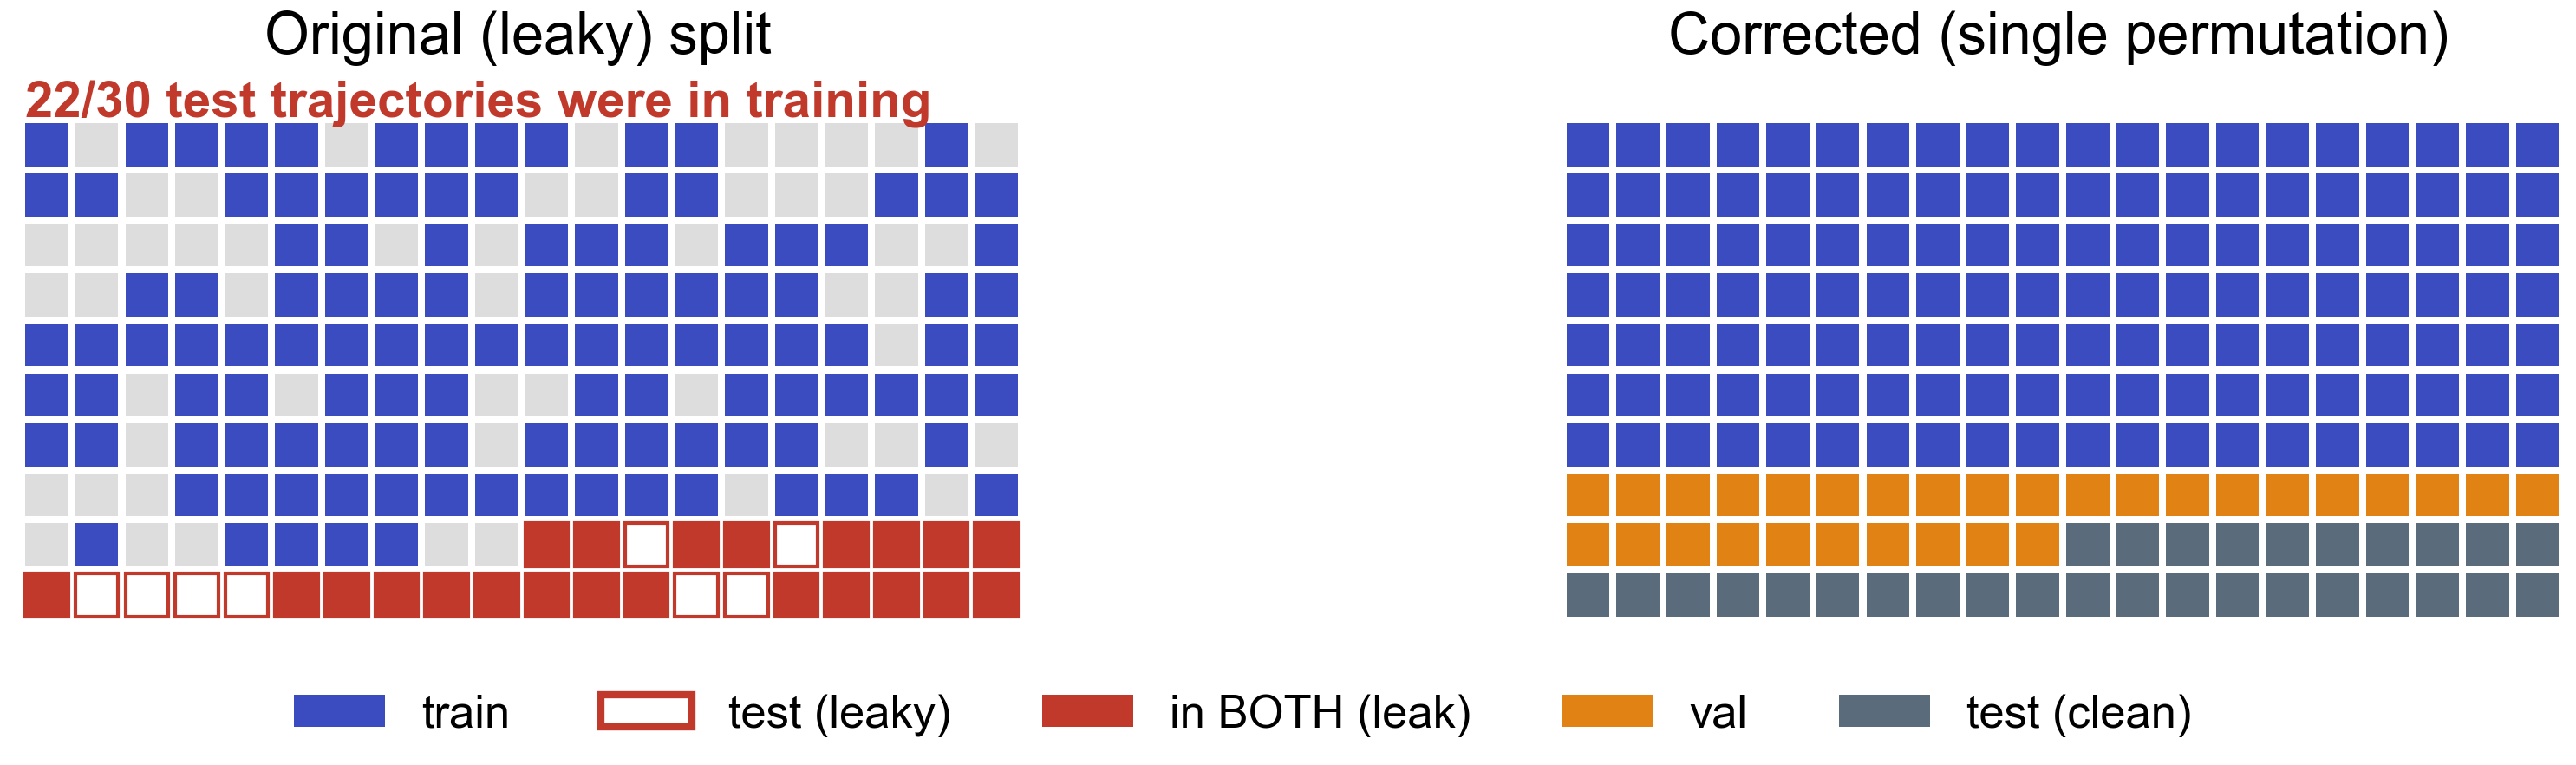
\includegraphics[width=0.92\textwidth]{figures/fig1_leakage_panel.png}
\caption{\scriptsize \textbf{The reported advantage originates in train--test leakage.} Trajectory-index membership for the $n=200$ pseudo-trajectories under the original (left) and corrected (right) splits. \emph{Left:} the model is trained on a permuted partition (blue) but evaluated on a contiguous tail slice (test, leaky); because the permuted training set spans $\sim$70\% of indices, $22$ of $30$ nominal test trajectories also appear in training (``in BOTH'', red). \emph{Right:} a single permutation yields disjoint train/validation/test blocks with no overlap. Only the Transformer was affected by the original asymmetry; all baselines were scored leakage-free.}
\label{fig:leakage}
\end{figure*}

\subsection{\textbf{Under a leakage-safe multi-seed protocol, the Transformer matches both baselines}}
\label{subsec:res_neural}

A single-seed estimate cannot distinguish a genuine effect from sampling variation introduced by pseudo-trajectory construction and model training. Repeating the full pipeline over $20$ seeds, each perturbing both randomness sources, yields the distributions in Fig.~\ref{fig:raincloud}A and the paired comparisons in Fig.~\ref{fig:forest} (neural). All three models occupy the same MAE range: Ridge $0.1774\pm0.0204$, the complexity-matched random forest $0.1794\pm0.0208$, and the Transformer $0.1787\pm0.0203$ (mean\,$\pm$\,s.d.\ over seeds). The paired differences against the Transformer are negligible and non-significant---Ridge $\overline{\Delta}=-0.0013$ ($d_z=-0.14$, $p=0.996$) and random forest $\overline{\Delta}=+0.0007$ ($d_z=+0.07$, $p=0.996$, Holm-corrected)---with $95\%$ confidence intervals on $\overline{\Delta}$ contained well within the pre-specified equivalence margin of $|\Delta|<0.01$ (Fig.~\ref{fig:forest}). The comparisons therefore support equivalence rather than merely failing to reject a difference.

Two features of Fig.~\ref{fig:raincloud}A are worth noting. First, the three per-seed distributions are mutually superimposed, so no model is reliably ranked above another. Second, the seed-to-seed spread (s.d.\ $\approx 0.020$) is an order of magnitude larger than any between-model mean difference ($\le 0.0013$), which is precisely why a single-seed comparison was able to report a spurious ranking: the reported gap was smaller than the noise it was drawn from.

The random forest here is tuned per seed by nested cross-validation over tree depth and leaf size, holding it to the same fair-complexity standard later applied to the mechanistic model (Sec.~\ref{subsec:res_ode}). An under-regularized fixed-depth forest appears modestly worse, but this reflects overfitting of a high-capacity learner on a small, near-linear task rather than any Transformer advantage; the regularized forest converges to the linear baseline.

\subsection{\textbf{The equivalence replicates on an independent cardiac lineage}}
\label{subsec:res_cardiac}

To distinguish a property of the task from a property of the neural dataset, the identical protocol was applied to an independent iPSC$\rightarrow$cardiomyocyte series (Sec.~\ref{subsec:data_state}). The equivalence replicates exactly (Fig.~\ref{fig:raincloud}B, Fig.~\ref{fig:forest} cardiac): Ridge $0.1100\pm0.0155$, random forest $0.1121\pm0.0175$, and Transformer $0.1100\pm0.0198$, with paired differences against the Transformer of $\overline{\Delta}\approx0$ for Ridge ($p=1.000$) and $+0.0021$ for the random forest ($d_z=+0.15$, $p=1.000$). Both intervals again fall within the equivalence margin. Across the two lineages and $40$ seeds, no model significantly outperforms the simplest linear baseline.

\begin{figure*}[!htbp]
\centering
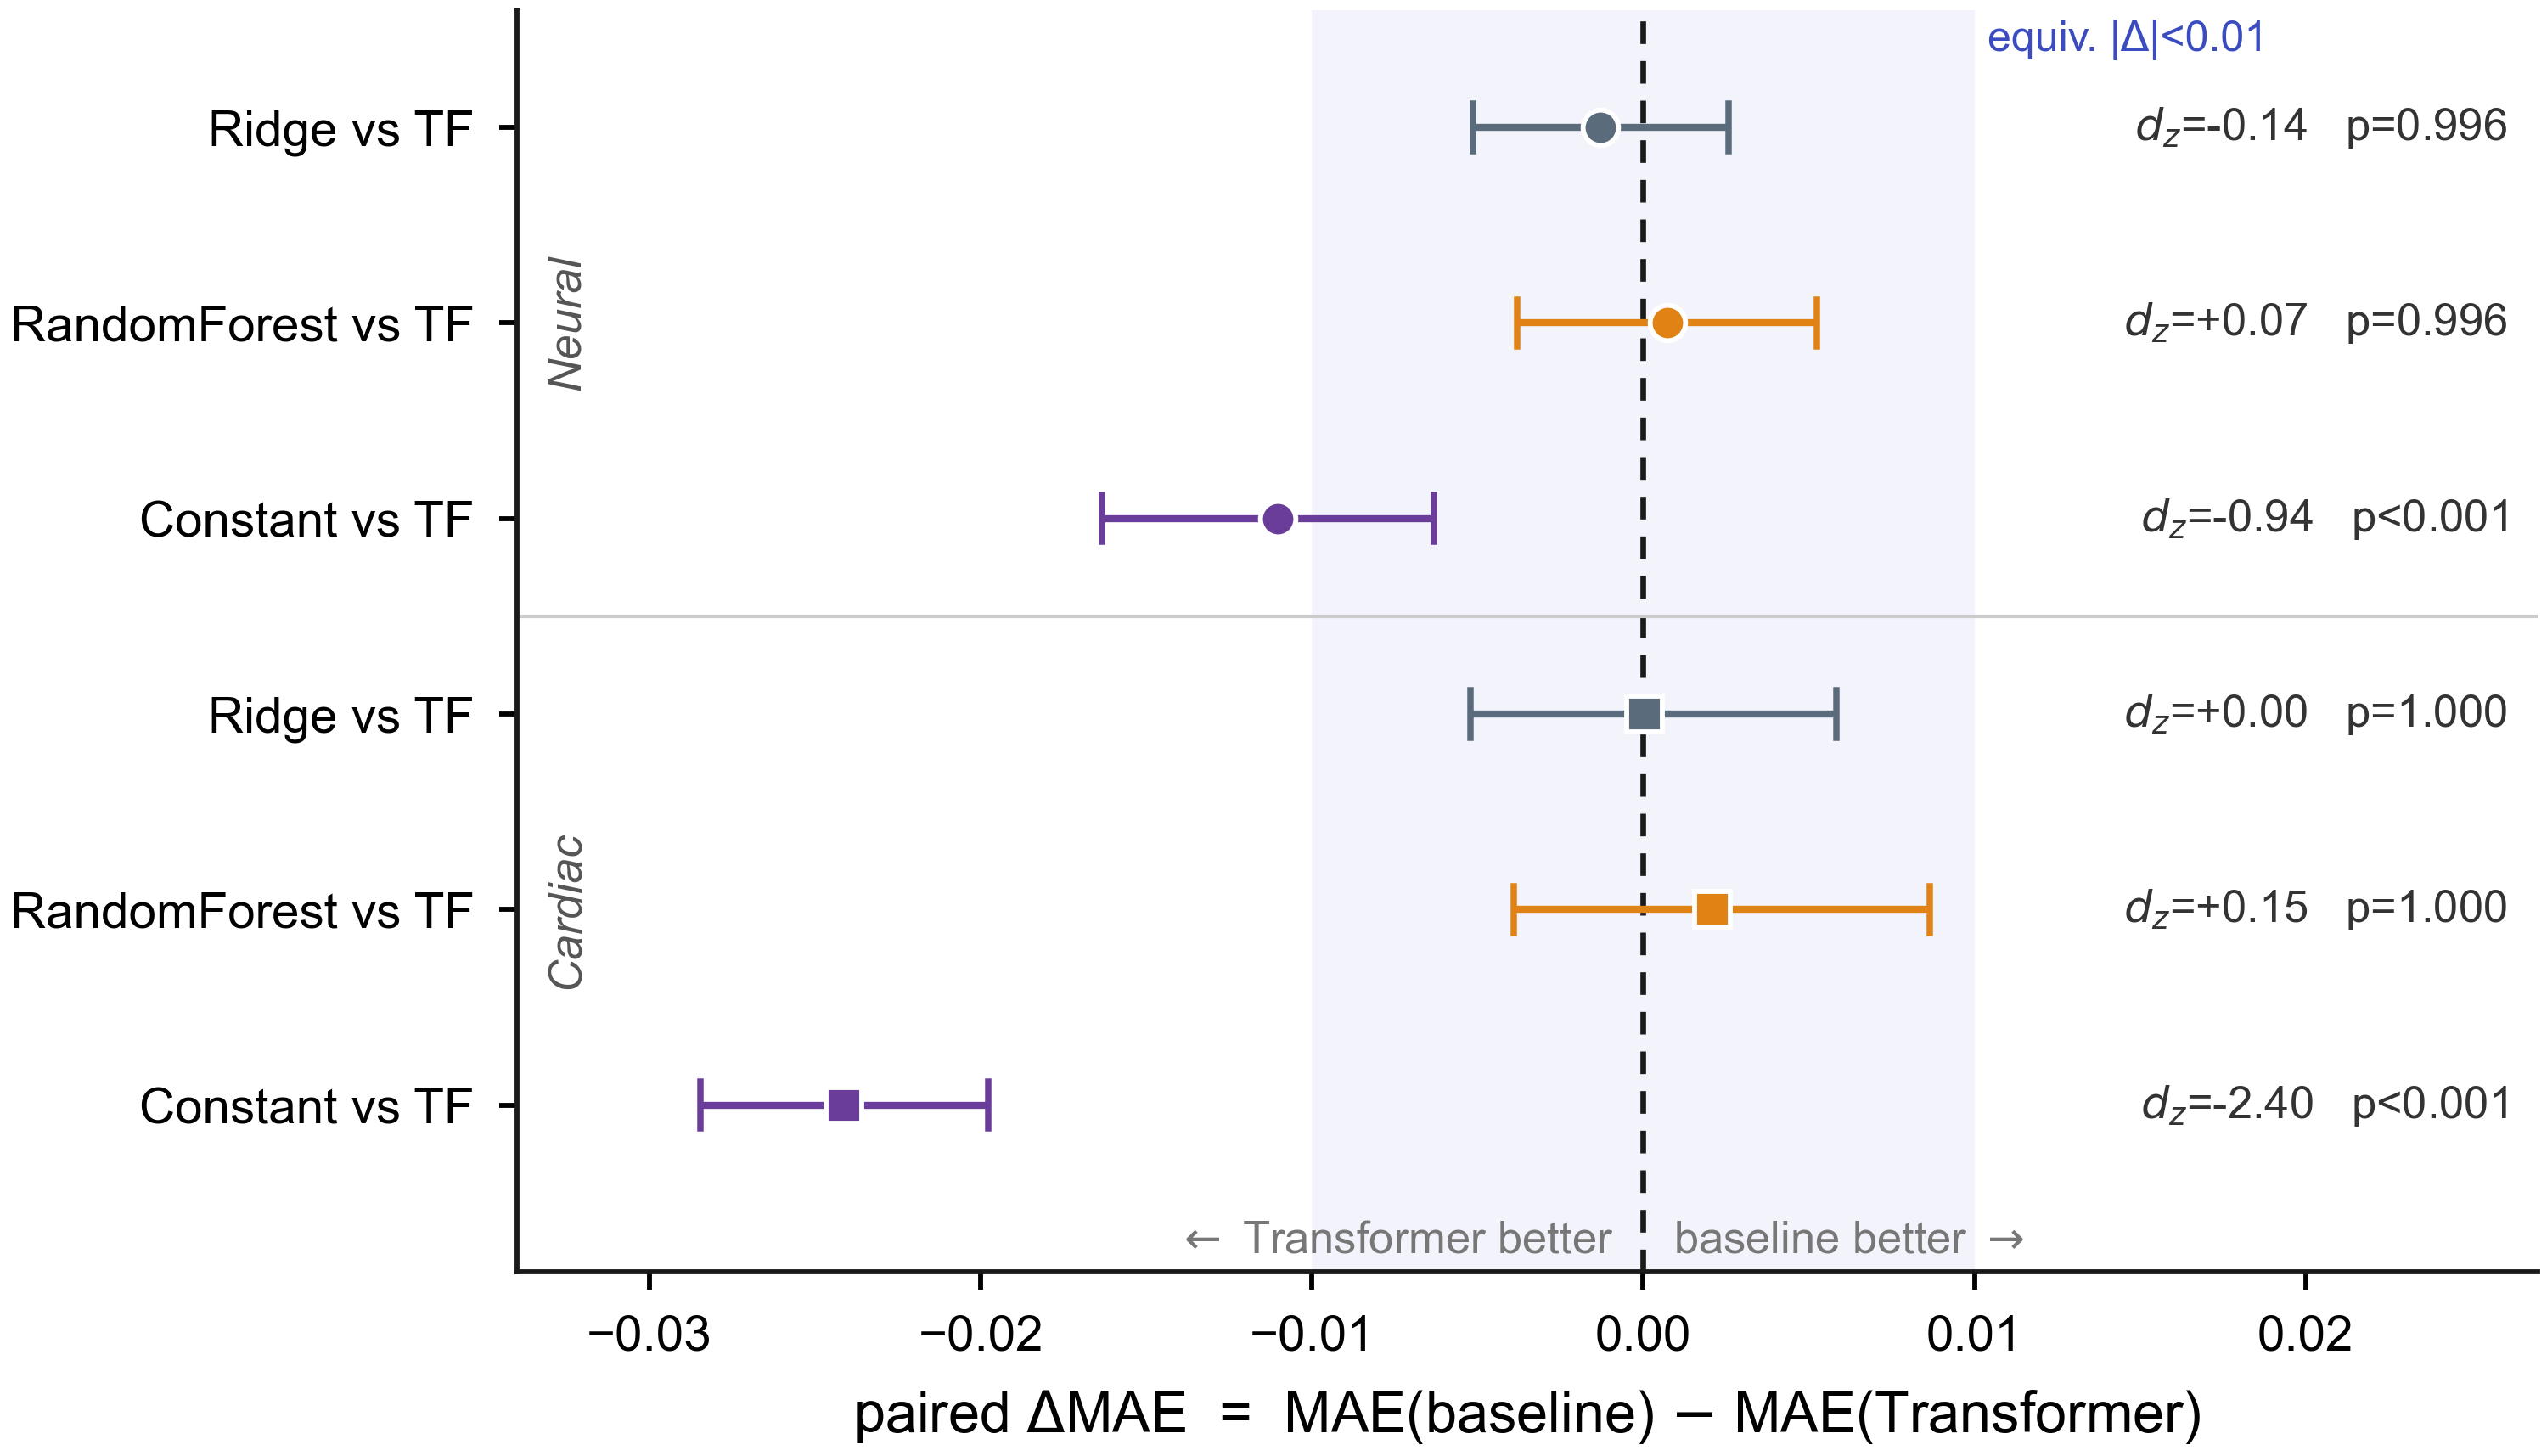
\includegraphics[width=0.82\textwidth]{figures/fig2_forest.png}
\caption{\scriptsize \textbf{All paired comparisons fall within the equivalence margin on both lineages.} Per-seed paired difference $\Delta=\mathrm{MAE}_{\text{baseline}}-\mathrm{MAE}_{\text{Transformer}}$ ($n=20$ seeds) with percentile paired-bootstrap $95\%$ confidence intervals; positive values favour the Transformer's competitors. Annotations give Cohen's $d_z$ and Holm-corrected Wilcoxon signed-rank $p$. The shaded band marks the equivalence region $|\Delta|<0.01$. Every interval, for both Ridge and the complexity-matched random forest and on both the neural and cardiac lineages, lies within the band, supporting statistical equivalence rather than non-detection of a difference.}
\label{fig:forest}
\end{figure*}

\begin{figure*}[!htbp]
\centering
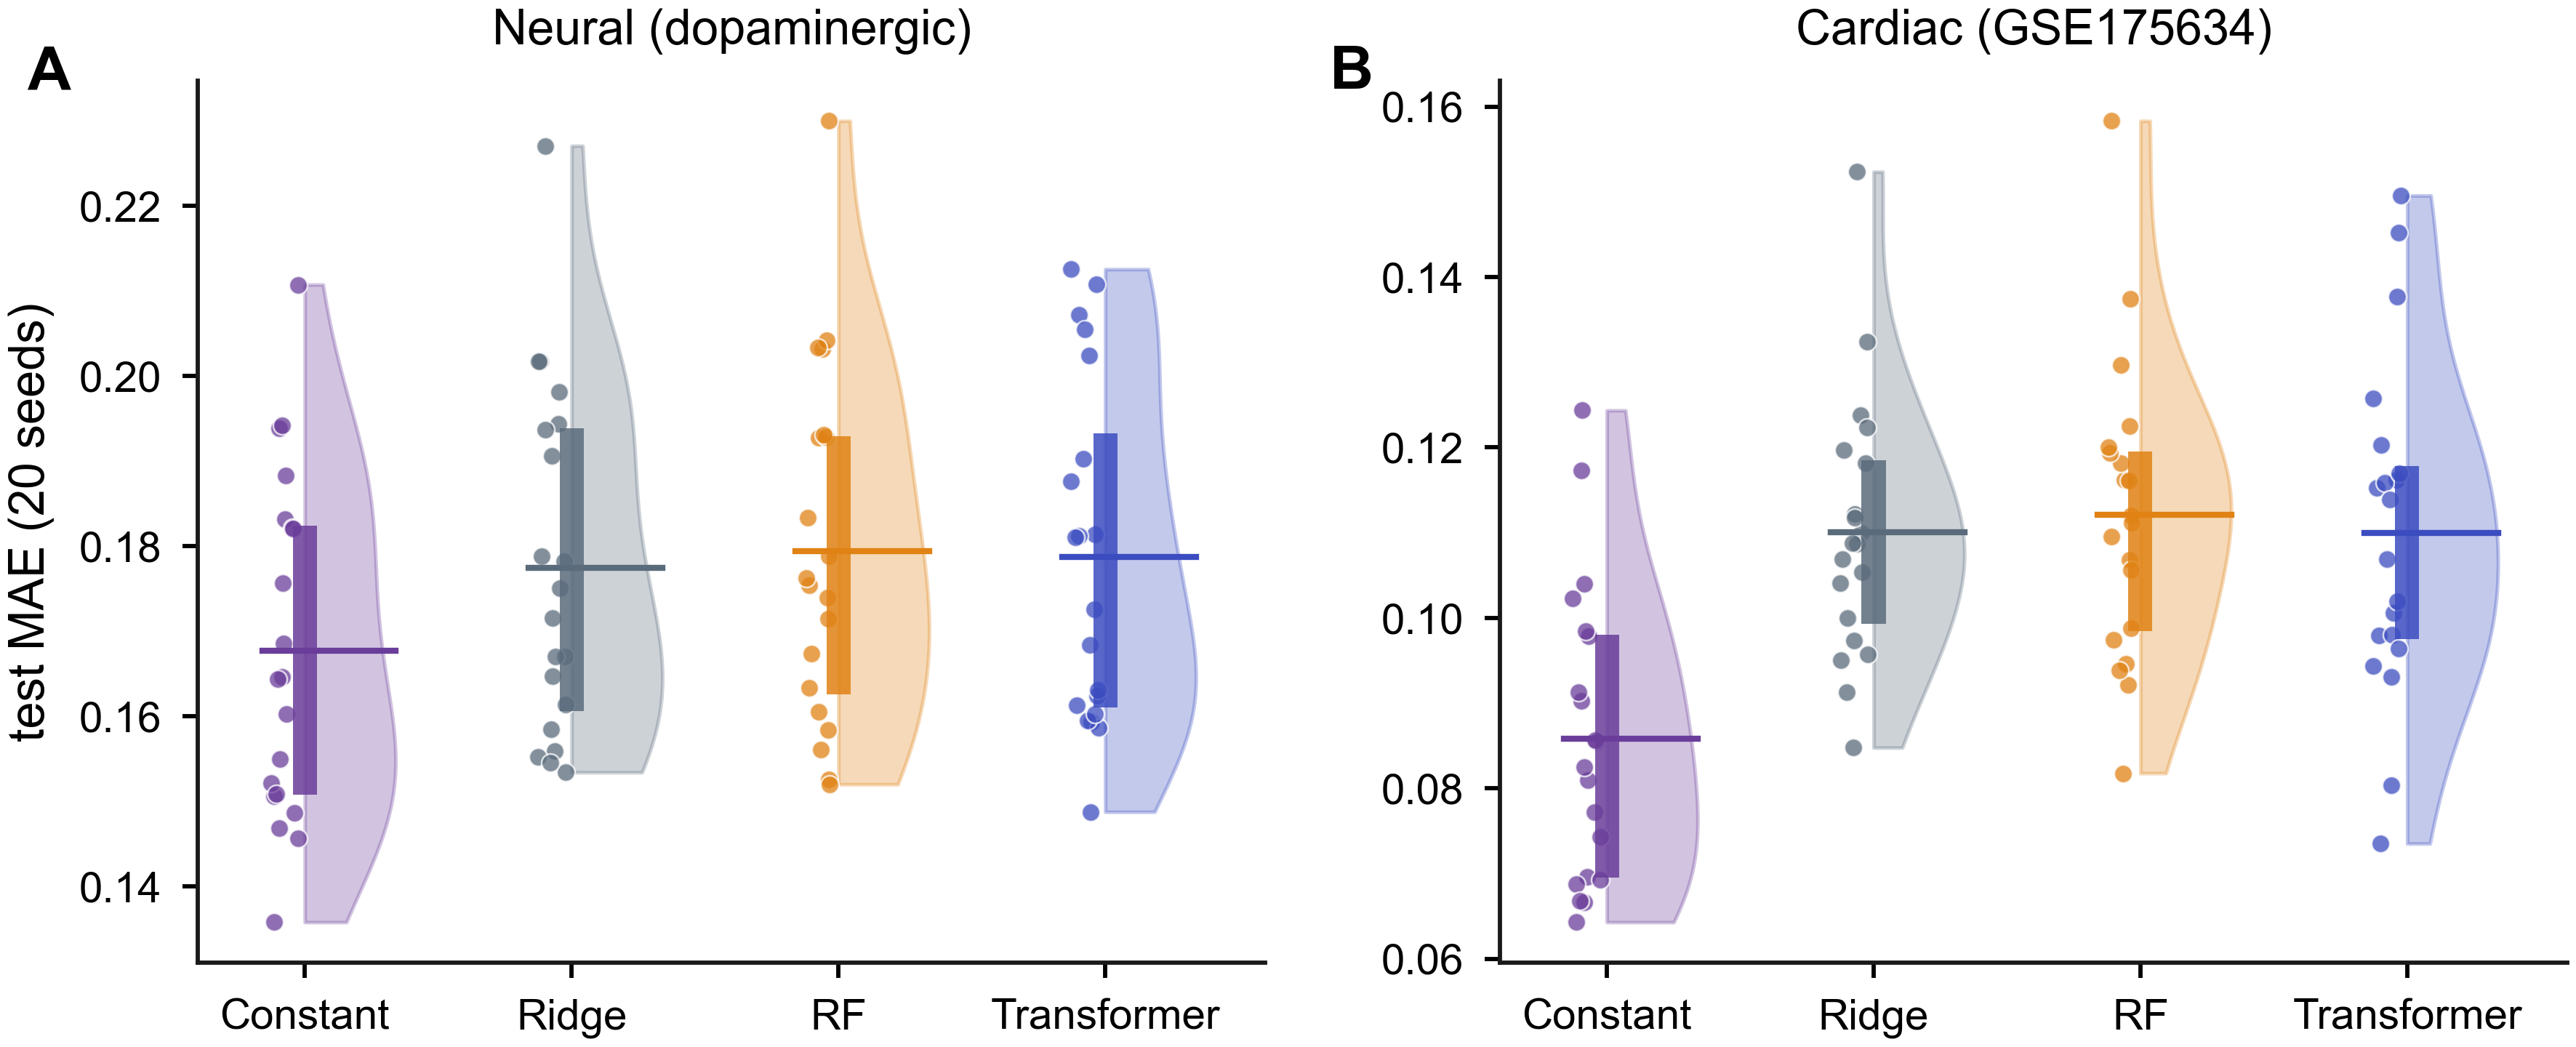
\includegraphics[width=0.92\textwidth]{figures/fig3_raincloud.png}
\caption{\scriptsize \textbf{Per-seed error distributions are mutually superimposed.} Test MAE over $n=20$ seeds for Ridge, the complexity-matched random forest, and the Transformer on the neural \textbf{(A)} and cardiac \textbf{(B)} lineages, shown as half-violin density, jittered per-seed points, and per-model mean (horizontal line). The three distributions overlap almost completely, and the seed-to-seed spread (s.d.\ $\approx0.020$ neural, $\approx0.017$ cardiac) dwarfs every between-model mean difference ($\le0.0021$), illustrating why a single-seed comparison cannot resolve a reliable ranking.}
\label{fig:raincloud}
\end{figure*}

\subsection{\textbf{The Transformer extracts no temporal structure}}
\label{subsec:res_temporal}

If the Transformer were exploiting the stage ordering of the input, destroying that ordering should degrade its accuracy. It does not. Permuting the stage order within each input context (shuffle) or removing the positional encoding (no-PE) leaves test MAE unchanged on both lineages (Fig.~\ref{fig:temporal}): shuffle-vs-ordered $\overline{\Delta}=-0.0002$ on the neural lineage ($p=0.87$) and $-0.0002$ on the cardiac lineage ($p=0.90$), with the no-PE ablation equally inert. The observed changes are of order $1$--$3\%$ of the seed-to-seed standard deviation, well inside the equivalence margin. The two channels through which temporal order can enter the prediction---positional encoding and self-attention over the ordered pair---therefore carry no usable signal.

This is the mechanistic core of the study. Because the pseudo-trajectories pair independently sampled cells across stages (Sec.~\ref{subsec:traj}), they contain no genuine within-trajectory temporal dependency for a sequence model to learn. The Transformer matches the linear baseline not because it fails to function---its training converges normally---but because the task as posed contains no temporal structure that distinguishes a sequence model from a memoryless regressor.

\begin{figure*}[!htbp]
\centering
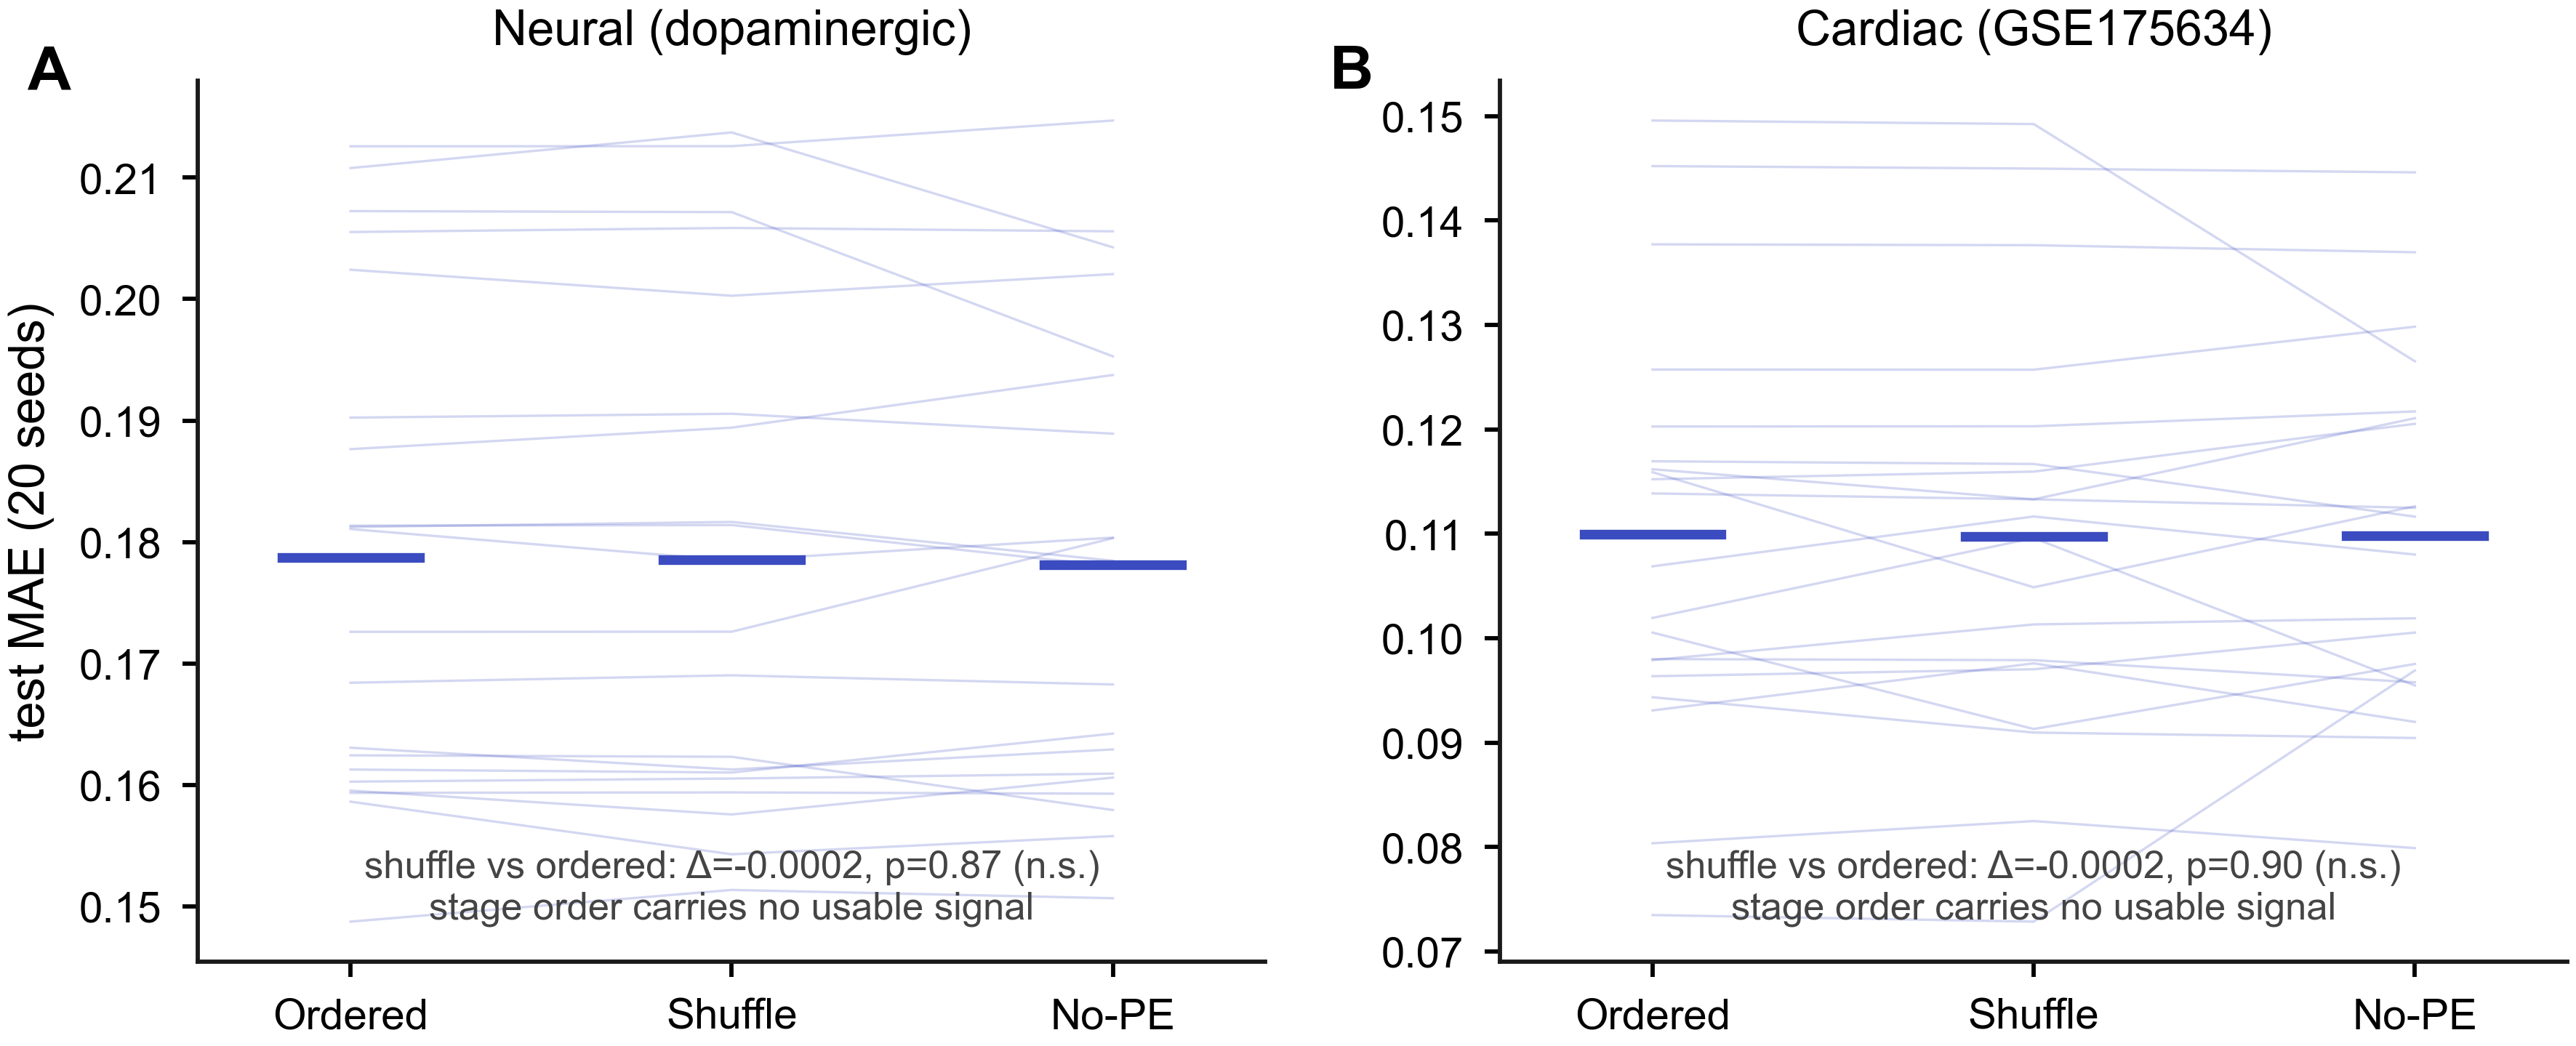
\includegraphics[width=0.92\textwidth]{figures/fig4_temporal.png}
\caption{\scriptsize \textbf{Destroying temporal order leaves accuracy unchanged.} Per-seed test MAE ($n=20$) for the Transformer under the ordered input, stage-order shuffle, and positional-encoding removal (no-PE) on the neural \textbf{(A)} and cardiac \textbf{(B)} lineages; faint lines are individual seeds and the bold bar is the per-condition mean. Shuffle-vs-ordered paired differences are $\overline{\Delta}=-0.0002$ ($p=0.87$, neural) and $-0.0002$ ($p=0.90$, cardiac), of order $1$--$3\%$ of the seed-to-seed standard deviation. The positional encoding and self-attention---the only routes by which stage order can enter the prediction---carry no usable signal.}
\label{fig:temporal}
\end{figure*}

\subsection{\textbf{A fairly calibrated mechanistic model provides no sample-level value}}
\label{subsec:res_ode}

A mechanistic ODE might still encode useful dynamical priors absent from the data-driven models. To test this fairly rather than against a deliberately weak baseline, the ODE was calibrated under three regimes of increasing sample-level fidelity (Sec.~\ref{subsec:ode_calib}) and evaluated on the same held-out trajectories. The result is monotone and holds on both lineages: the fairer the sample-level calibration, the worse the prediction (Fig.~\ref{fig:ode}). On the neural lineage the test MAE rises from $0.198$ (population-mean; $+12\%$ over Ridge) through $0.295$ (distributional; $+66\%$) to $0.370$ (per-trajectory; $+108\%$); on the cardiac lineage from $0.248$ ($+126\%$) through $0.258$ ($+135\%$) to $0.334$ ($+203\%$). Every regime, on both lineages, lies above the corresponding Ridge reference.

The monotonicity is the expected signature of the same mechanism identified in Sec.~\ref{subsec:res_temporal}. Per-trajectory calibration grants the ODE the most freedom to fit each test trajectory's early step, but because the trajectories pair independent cells, that early step carries no information about the late state; the additional freedom fits noise and generalizes worse. Population-calibrated mechanistic priors thus provide no sample-level predictive value here, and increasing their sample-level fidelity actively harms forecasting. (This is a statement about population-level priors on pseudo-trajectory data, not a general verdict on mechanistic modeling.)

\begin{figure}[!htbp]
\centering
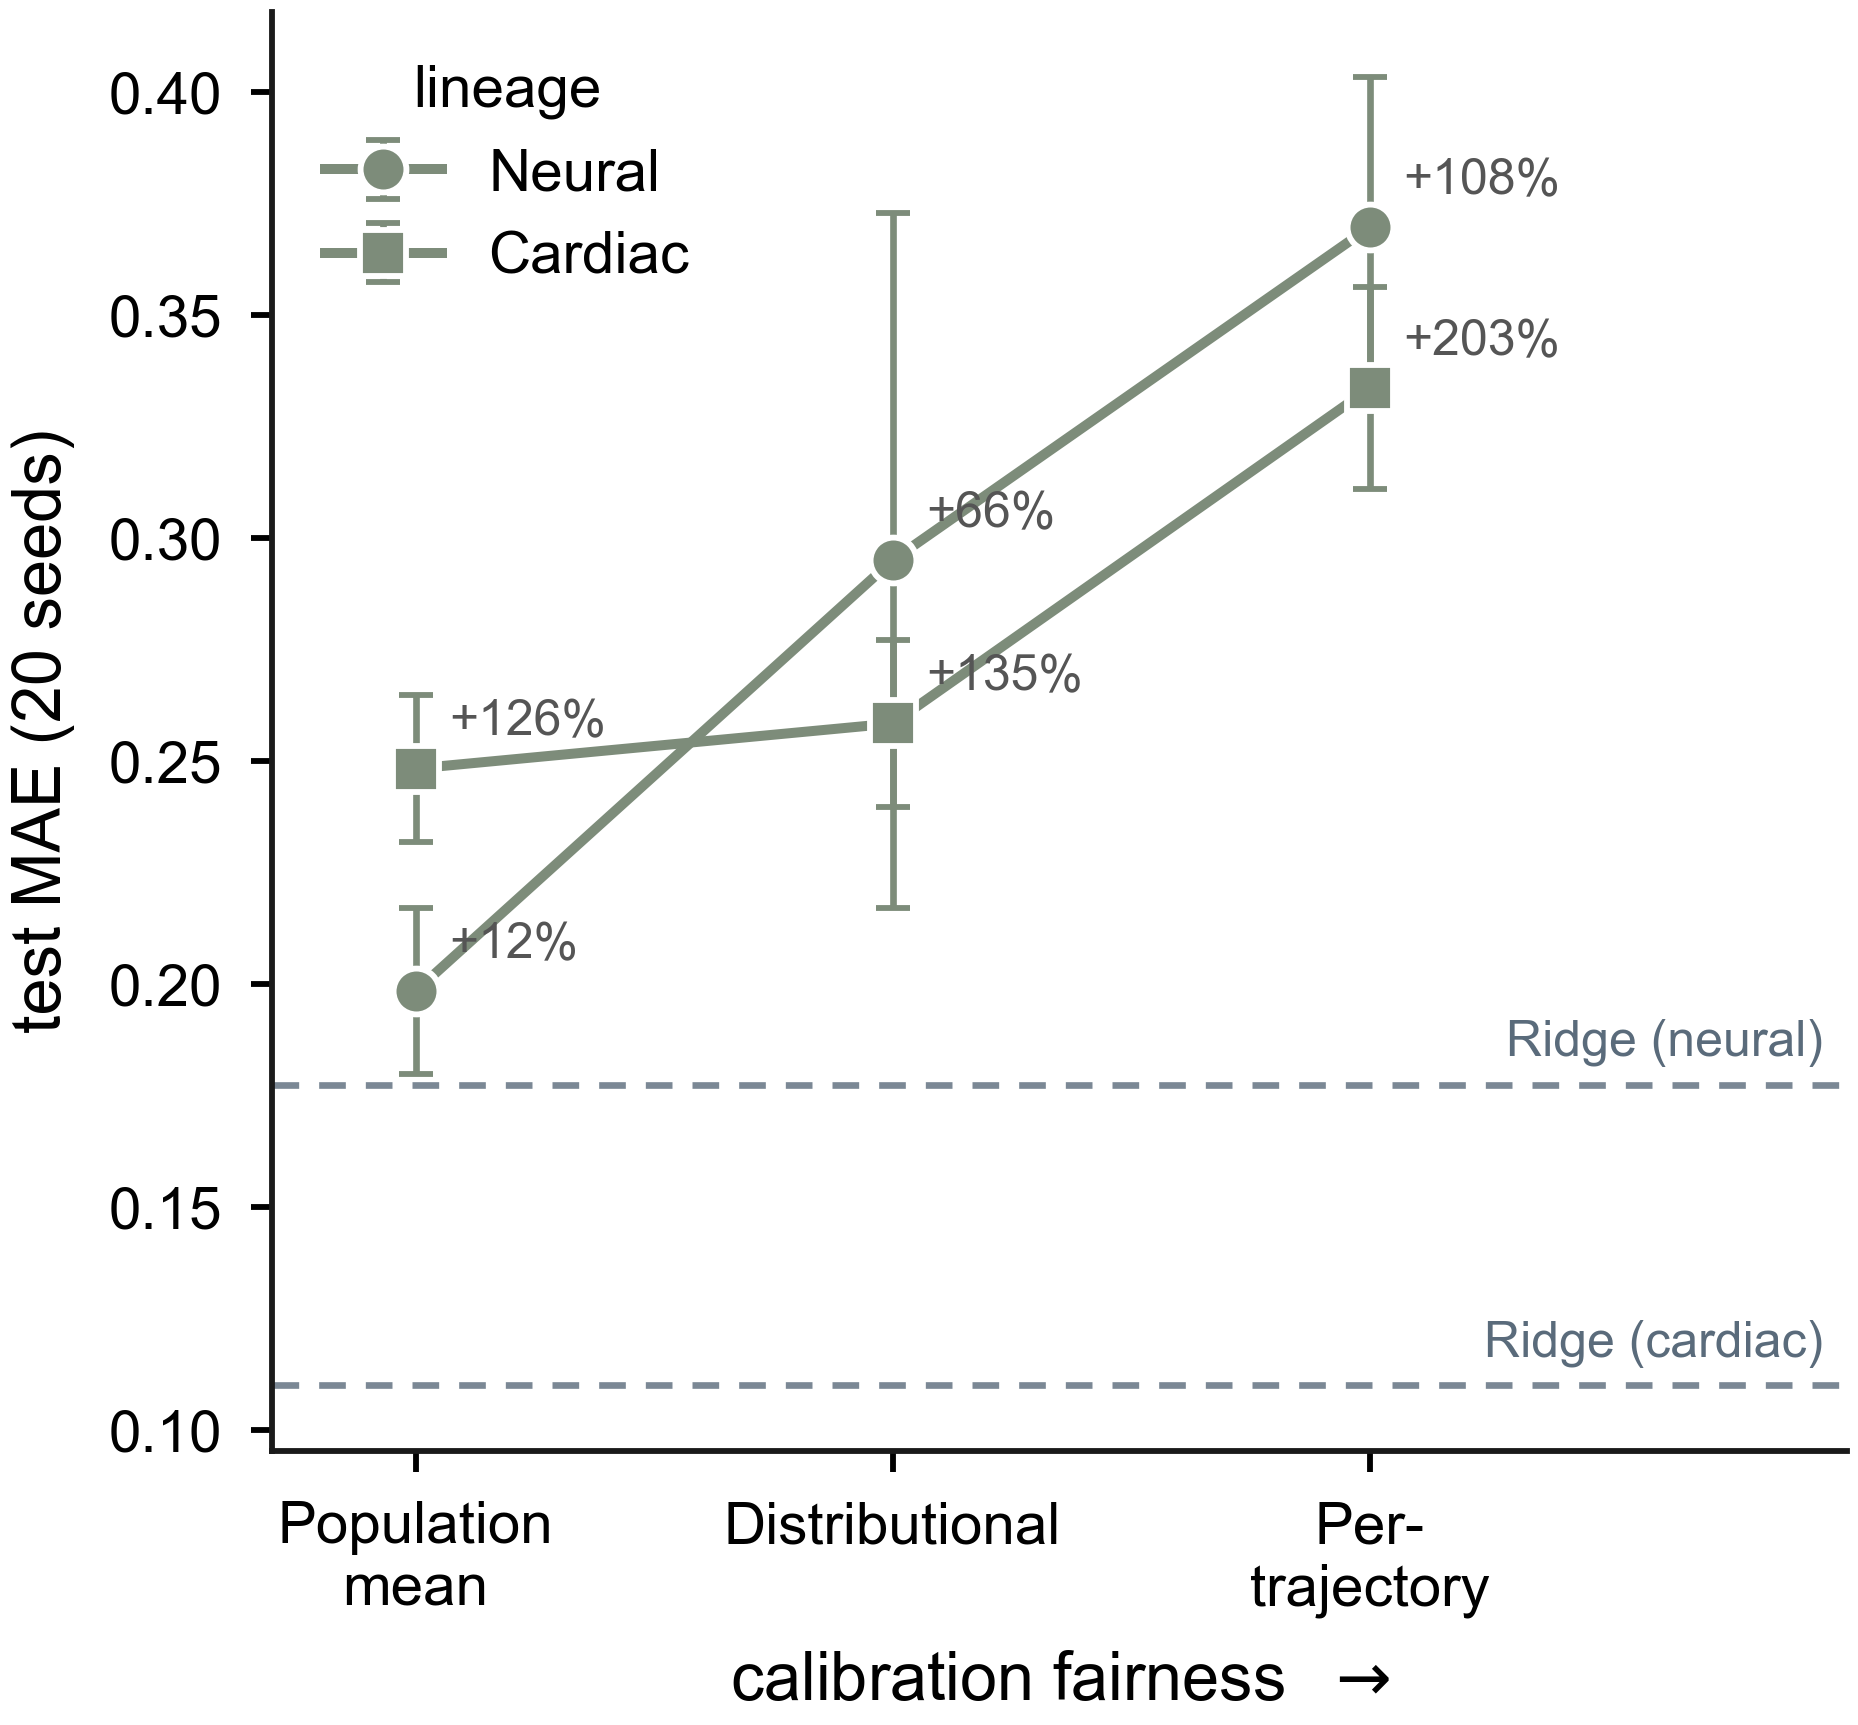
\includegraphics[width=0.86\columnwidth]{figures/fig5_ode.png}
\caption{\scriptsize \textbf{Fairer sample-level calibration of the mechanistic model worsens prediction.} Test MAE ($n=20$ seeds, mean with s.d.\ whiskers) of the mechanistic ODE under three calibration regimes of increasing sample-level fidelity, for the neural (circles) and cardiac (squares) lineages; annotations give the increase over the corresponding Ridge baseline (dashed references). Error rises monotonically from population-mean to per-trajectory calibration on both lineages, the expected consequence of granting added freedom to fit the noise of independently paired cells.}
\label{fig:ode}
\end{figure}

\subsection{\textbf{The null is robust to the state representation}}
\label{subsec:res_sensitivity}

Finally, to confirm that the equivalence does not hinge on the particular two-dimensional state, the Transformer-versus-Ridge comparison was recomputed across $38$ state-construction variants (leave-one-marker-out for every panel gene, median and $z$-score aggregation, and an enlarged neural panel), each over $20$ seeds (Fig.~\ref{fig:sensitivity}). The paired gap is centred near zero throughout (mean $+0.0004$, range $[-0.0016,+0.0028]$, maximum $|d_z|=0.19$), and \emph{no} variant produces a statistically significant Transformer advantage ($0/38$). The conclusion is a property of the forecasting task, not of any specific feature definition. Per-feature errors show the expected lineage-specific difficulty pattern---the differentiation score is harder to predict than the pluripotency score on the cardiac lineage, and the reverse on the neural lineage---but model identity does not affect either component.

\begin{figure}[!htbp]
\centering
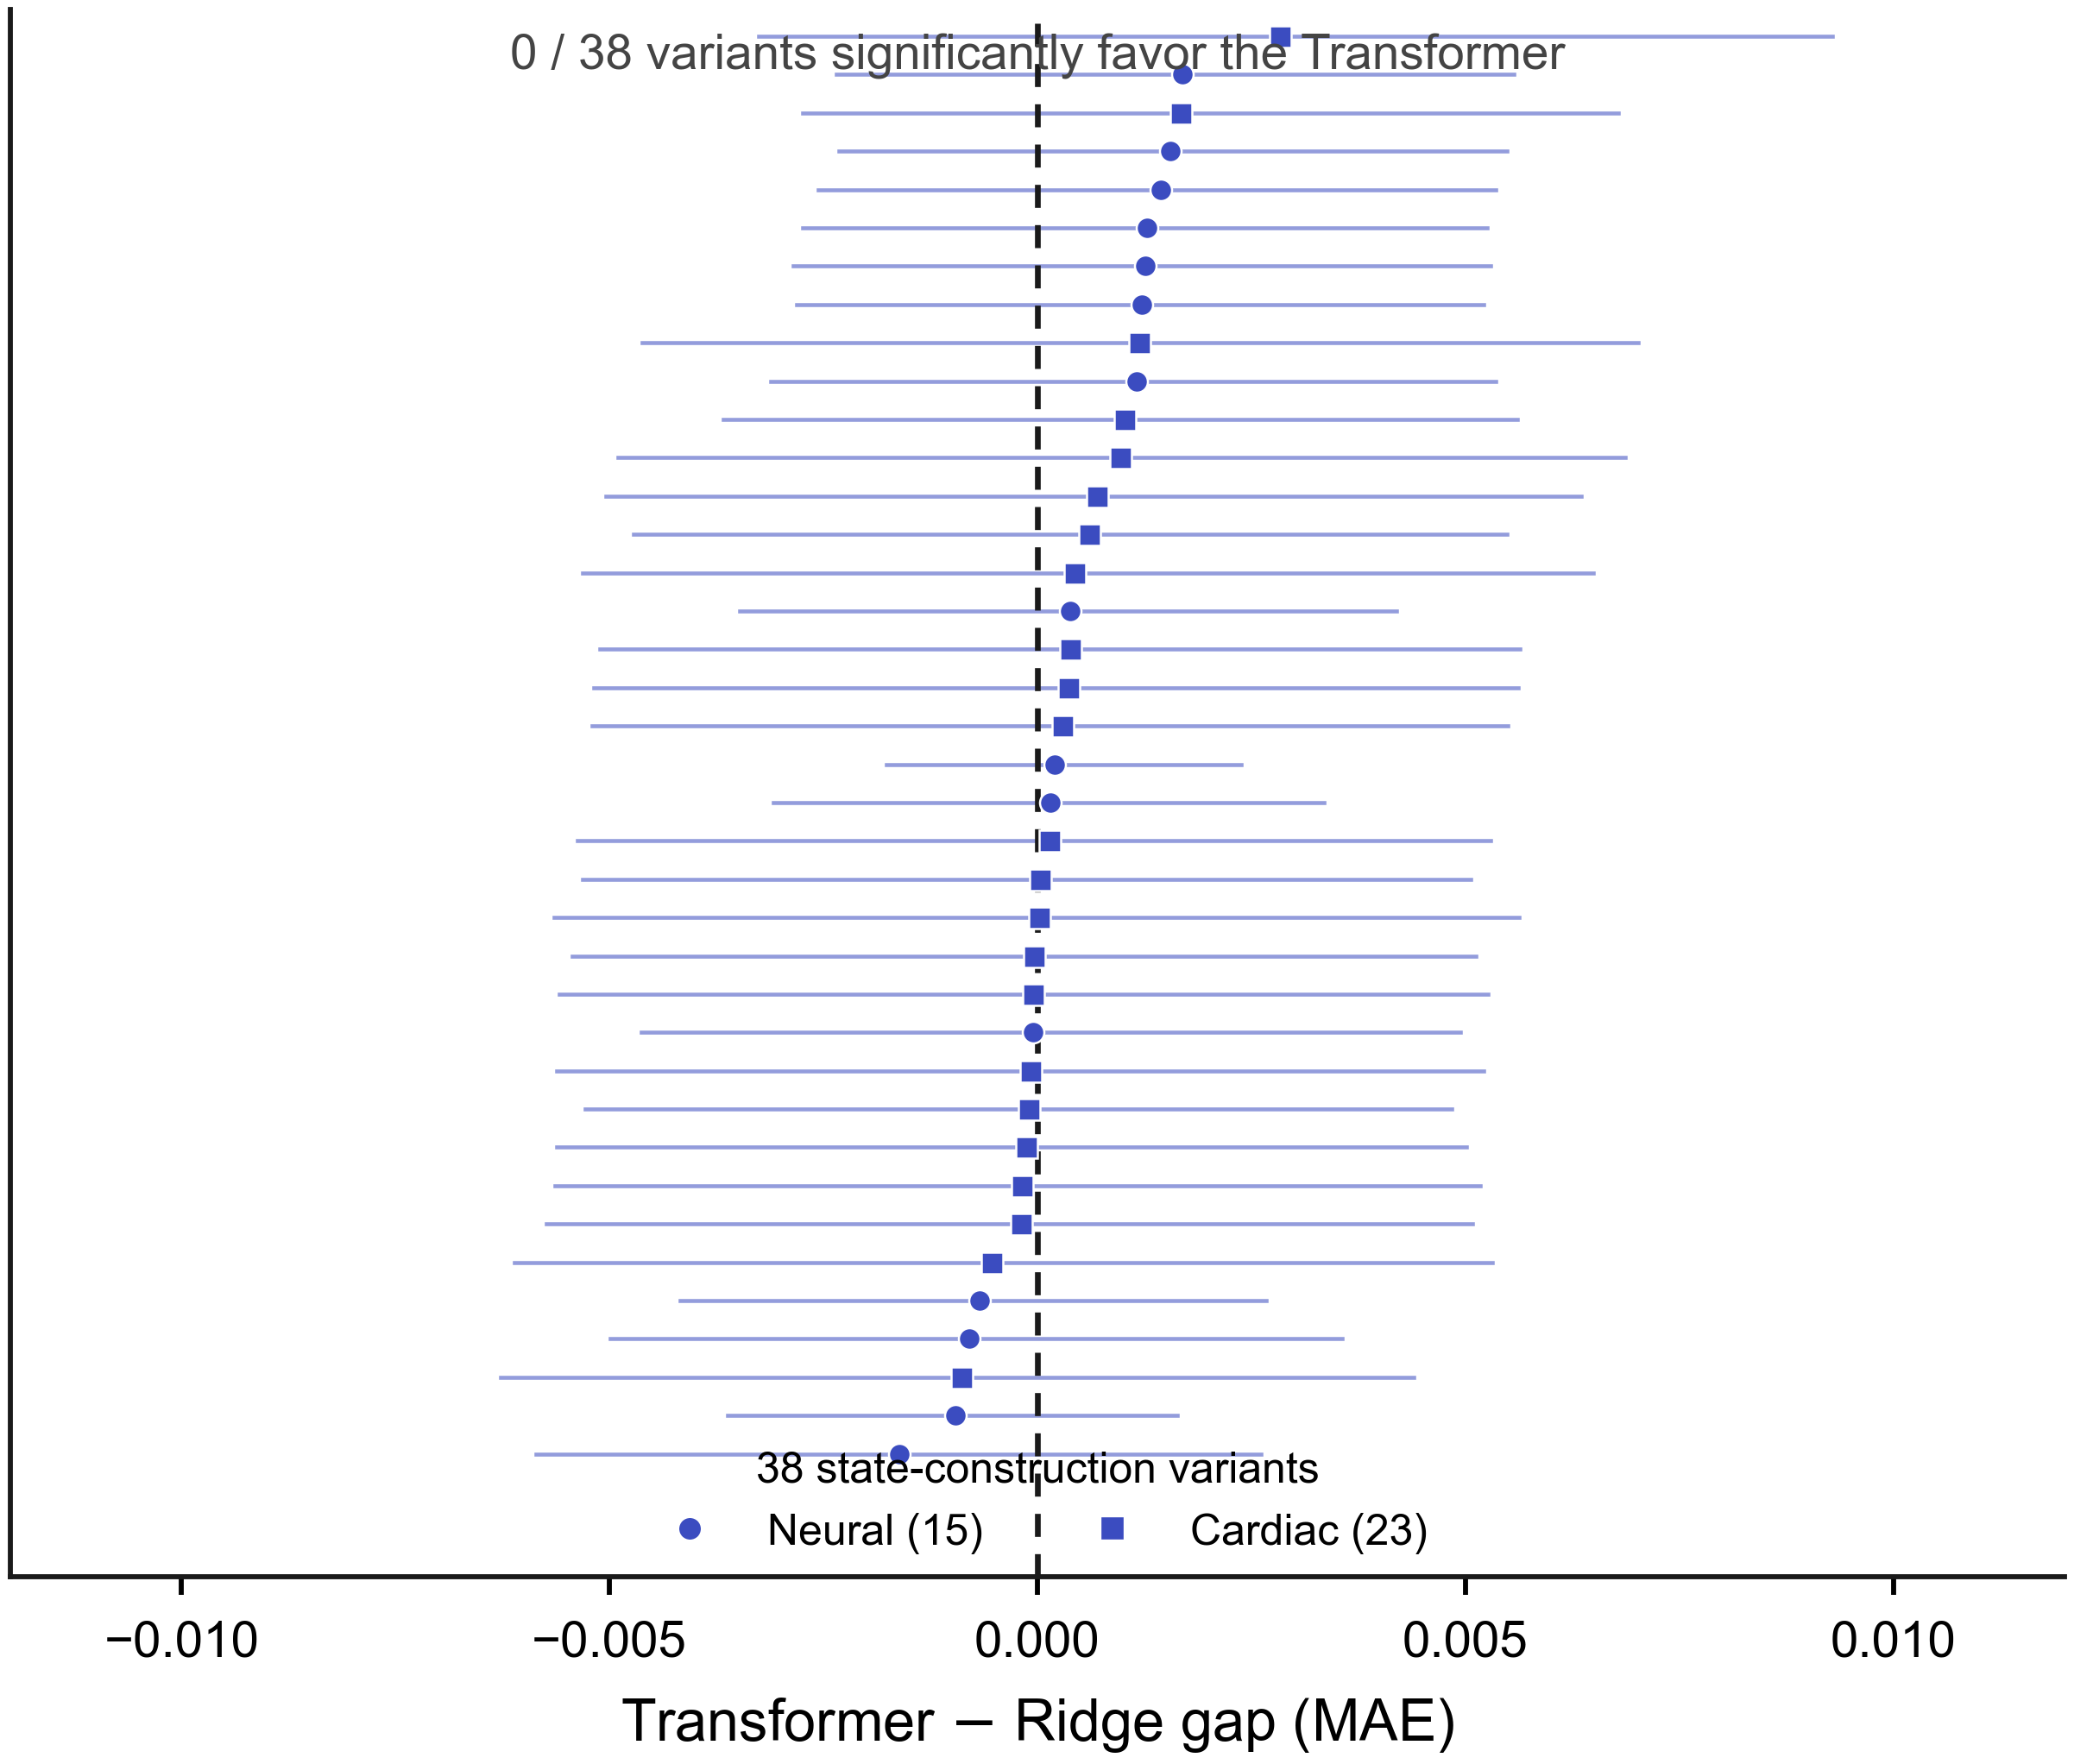
\includegraphics[width=0.86\columnwidth]{figures/fig6_sensitivity.png}
\caption{\scriptsize \textbf{The equivalence is invariant to the state representation.} Paired Transformer$-$Ridge MAE gap (point estimate with $95\%$ CI, $n=20$ seeds) for each of $38$ state-construction variants---per-gene leave-one-out, median and $z$-score aggregation, and an enlarged neural panel---sorted by gap; circles, neural ($15$ variants); squares, cardiac ($23$). Every interval lies within the equivalence margin $|\Delta|<0.01$ and no variant significantly favours the Transformer ($0/38$), establishing the result as a property of the task rather than of any particular feature definition.}
\label{fig:sensitivity}
\end{figure}

\section{\textbf{Discussion}}
\label{sec:discussion}

This study set out to determine whether a Transformer provides a genuine advantage for discrete-stage differentiation forecasting from single-cell data. The answer, established under a leakage-safe and statistically resolved protocol, is that it does not: across two differentiation lineages and $40$ random seeds, the Transformer is statistically equivalent to both an ten-parameter linear model and a complexity-matched random forest. The $+19.4\%$ advantage obtained under a leaky, single-seed evaluation inverted to a $2\%$ deficit once the evaluation was corrected.

\subsubsection{One mechanism explains every result.} The findings are not a collection of independent negatives but a single causal story. The pseudo-trajectory construction---standard in this literature---pairs independently sampled cells across stages, because cross-sectional scRNA-seq provides no lineage tracing. This destroys any within-trajectory temporal dependency, so the conditional distribution of the late state given the two earlier states reduces to a smooth, near-linear map for which a memoryless regressor is optimal. Every result follows from this. The Transformer matches the linear model because there is no temporal structure to exploit (Fig.~\ref{fig:forest}); destroying stage order changes nothing because order was never informative (Fig.~\ref{fig:temporal}); and the mechanistic ODE worsens monotonically as calibration is made fairer because added flexibility fits the noise of independently paired cells rather than signal (Fig.~\ref{fig:ode}). The same excess-flexibility-fits-noise effect explains why an under-regularized random forest appears worse until it is properly regularized. A high-capacity model on this task is, at best, harmless and, at worst, actively misled.

\subsubsection{This is not an indictment of Transformers.} The Transformer trains stably and predicts as well as any model considered; it simply has no structural advantage to express on data that lack the dependency it is designed to capture. The difficulty lies not in the choice of architecture but in evaluating any expressive model on a task whose construction precludes the very signal the architecture targets---a difficulty compounded, when present, by leakage and single-seed reporting that together can manufacture an apparent gain. These are evaluation failures, and they are correctable.

\subsubsection{Implications for single-cell forecasting practice.} Three practices would have surfaced the problem immediately and are inexpensive to adopt. First, leakage-safe evaluation with a single, consistent split shared identically across models; the asymmetry here arose entirely from an inconsistency affecting only one model. Second, multi-seed reporting with paired effect sizes and equivalence reasoning rather than single-seed point estimates; the spurious ranking was smaller than the seed-to-seed noise it was drawn from, and no honest comparison at $n=1$ seed was possible. Third, and most specific to this setting, a temporal-order control---shuffling the stage order---whenever ``forecasting'' is claimed on pseudo-trajectories; if shuffling does not degrade performance, the temporal framing is unsupported regardless of how sophisticated the model is. The linear model is the natural baseline-of-record for this class of task, since it bounds the achievable accuracy and any complex model must be shown to exceed it under these controls.

\subsubsection{Limitations and scope.} The conclusions are specific to forecasting tasks built on pseudo-trajectories from cross-sectional data; they do not bear on settings with genuine lineage tracing (e.g.\ lineage-barcoded or metabolically labeled time-series), where real within-cell temporal dependency exists and a sequence model may have something to learn. Establishing whether deep temporal models add value in those settings is the natural next step, and the protocol used here---leakage-safe splits, multi-seed paired statistics, and an explicit temporal-order control---transfers directly to it. The two-dimensional marker-program state is also a deliberate simplification; the representation-sensitivity analysis (Fig.~\ref{fig:sensitivity}) shows the equivalence is robust to reasonable choices within that family, but richer learned representations on lineage-resolved data remain unexamined here.

\section{\textbf{Conclusion}}
\label{sec:conclusion}
Across two independent differentiation lineages and forty random seeds, a Transformer proved statistically equivalent to an ten-parameter linear model and a complexity-matched random forest for discrete-stage forecasting from single-cell data. An advantage seen under conventional single-seed evaluation was traced to train-test leakage that reversed once corrected. A single mechanism explains this. Because single-cell measurement is destructive, the pseudo-trajectories underlying such forecasts concatenate independently sampled cells and carry no temporal dependency. This is confirmed by controls where shuffling stage order or removing positional encoding leaves accuracy unchanged, and by a mechanistic ODE that degrades as its calibration is made fairer. Therefore, a memoryless predictor is optimal and added capacity fits noise rather than dynamics. The lasting contribution is methodological rather than architectural. A leakage-safe split shared across models, multi-seed paired statistics with explicit equivalence testing, a temporal-order control that tests rather than assumes dynamical signal, and cross-lineage replication together form an inexpensive, transferable template for any claim to forecast cellular state from cross-sectional snapshots. In single-cell machine learning, such rigor is not an obstacle to demonstrating genuine progress but its precondition. Only an evaluation that can fail to find an effect can credibly claim to have found one.

 

\section{\textbf{Availability of data and materials}}

The dopaminergic-neuron differentiation scRNA-seq data are from~\cite{jerber2021population}. Open-access count data are available in the European Nucleotide Archive (ENA) under study accession ERP121676 (BioProject PRJEB38269; https://www.ebi.ac.uk/ena/browser/view/PRJEB38269); genotype-linked data are under managed access in the European Genome–phenome Archive (EGA) under study EGAS00001002885; and processed per-timepoint count files are deposited on Zenodo (https://zenodo.org/record/4333872). The cardiomyocyte differentiation data are available from the Gene Expression Omnibus under accession GSE175634 (https://www.ncbi.nlm.nih.gov/geo/query/acc.cgi?acc=GSE175634)~\cite{elorbany2022single}. No new sequencing data were generated in this study.
All source code required to reproduce the analyses, figures, and tables — including the leakage-safe trajectory construction, the multi-seed evaluation pipeline, all model implementations, and the per-seed metric outputs from which every reported value is derived — is openly available at https://github.com/xaviwho/leakage-safe-benchmark. The repository includes pinned dependency specifications, the derived per-seed result files, and scripts that regenerate each figure and table directly from those files. The code is released under the [MIT/Apache-2.0] license.
Project name: Leakage-Safe Benchmark for Single-Cell Differentiation Forecasting

Project home page: https://github.com/xaviwho/leakage-safe-benchmark

Operating system(s): Platform independent

Programming language: Python 3.14

Other requirements: [pinned versions from requirements.txt — e.g. PyTorch, Scanpy, SciPy, scikit-learn, NumPy]

License: [MIT / Apache-2.0]

Any restrictions to use by non-academics: None
%Highlight potential areas for future work, possibly mentioning how this foundation can support efforts to improve reproducibility

\vspace{-0.2cm}
\small
\section *{Acknowledgment } 
This work was partly supported by Innovative Human Resource Development for Local Intellectualization program through the IITP grant funded by the Korea government (MSIT) (IITP-2026-RS-2020-II201612, 25\%) and by Priority Research Centers Program through the NRF funded by the MEST (2018R1A6A1A03024003, 25\%) and by the MSIT, Korea, under the ITRC support program (IITP-2026-RS-2024-00438430, 25\%) and by Basic Science Research Program through the National Research Foundation of Korea(NRF) funded by the Ministry of Education(RS-2025-25431637, 25\%).

\bibliography{sn-bibliography}
\end{document}
